%% LyX 2.4.0~RC3 created this file.  For more info, see https://www.lyx.org/.
%% Do not edit unless you really know what you are doing.
\documentclass[journal,article,submit,pdftex,moreauthors]{Definitions/mdpi}
\usepackage[utf8]{inputenc}
\usepackage{float}
\usepackage{url}
\usepackage{amsmath}
\usepackage{graphicx}

\makeatletter

%%%%%%%%%%%%%%%%%%%%%%%%%%%%%% LyX specific LaTeX commands.

\Title{Gen2Gen: Efficiently training artificial neural networks using a series
of genetic algorithms}

\TitleCitation{Gen2Gen: Efficiently training artificial neural networks using a series
of genetic algorithms}

\Author{Ioannis G. Tsoulos$^{1,*}$, Vasileios Charilogis$^{2}$}

\AuthorNames{Tsoulos, I.G., Charilogis, V.}

\AuthorNames{Ioannis G. Tsoulos, Vasileios Charilogis }

\AuthorCitation{Tsoulos, I.G.; Charilogis, V.}


\address{$^{1}$\quad{}Department of Informatics and Telecommunications,
University of Ioannina, Greece; itsoulos@uoi.gr\\
$^{2}$\quad{}Department of Informatics and Telecommunications, University
of Ioannina, Greece; v.charilog@uoi.gr}


\corres{Correspondence: itsoulos@uoi.gr}


\abstract{Artificial neural networks have been used in a multitude of applications
in various research areas in recent decades, providing excellent results
in both data classification and data fitting. Their success is based
on the effective identification (training) of their parameters using
optimization techniques, and hence a series of programming methods
have been developed for training these models. However, many times
these techniques either can identity only some local minima of the
error function with poor overall results or present overfitting problems
in which the performance of the artificial neural network is significantly
reduced when it is applied on different data from the training set.
This manuscript introduces a method for the efficient training of
artificial neural networks, where a series of genetic algorithms is
applied to the network parameters in several stages. In the first
stage, an initial identification of the network value interval is
made, in the second stage, the initial estimate of the value interval
is improved, and in the third stage, the final adjustment of the network
parameters within the previously identified value interval takes place.
The new method was tested on some classification and regression problems
found in the relevant literature, and the experimental results was
compared against the results obtained by the application of other
well - known methods used for neural network training.}


\keyword{Genetic algorithms; Evolutionary computation; Artificial neural networks}

\newcommand*\LyXZeroWidthSpace{\hspace{0pt}}
\DeclareTextSymbolDefault{\textquotedbl}{T1}
%% Because html converters don't know tabularnewline
\providecommand{\tabularnewline}{\\}
\floatstyle{ruled}
\newfloat{algorithm}{tbp}{loa}
\providecommand{\algorithmname}{Algorithm}
\floatname{algorithm}{\protect\algorithmname}

%%%%%%%%%%%%%%%%%%%%%%%%%%%%%% User specified LaTeX commands.
%  LaTeX support: latex@mdpi.com 
%  For support, please attach all files needed for compiling as well as the log file, and specify your operating system, LaTeX version, and LaTeX editor.

%=================================================================
%\documentclass[preprints,article,submit,pdftex,moreauthors]{Definitions/mdpi} 
% For posting an early version of this manuscript as a preprint, you may use "preprints" as the journal. Changing "submit" to "accept" before posting will remove line numbers.

% Below journals will use APA reference format:
% admsci, behavsci, businesses, econometrics, economies, education, ejihpe, famsci, games, humans, ijcs, ijfs, journalmedia, jrfm, languages, psycholint, publications, tourismhosp, youth

% Below journals will use Chicago reference format:
% arts, genealogy, histories, humanities, jintelligence, laws, literature, religions, risks, socsci

%--------------------
% Class Options:
%--------------------
%----------
% journal
%----------
% Choose between the following MDPI journals:
% accountaudit, acoustics, actuators, addictions, adhesives, admsci, adolescents, aerobiology, aerospace, agriculture, agriengineering, agrochemicals, agronomy, ai, air, algorithms, allergies, alloys, amh, analytica, analytics, anatomia, anesthres, animals, antibiotics, antibodies, antioxidants, applbiosci, appliedchem, appliedmath, appliedphys, applmech, applmicrobiol, applnano, applsci, aquacj, architecture, arm, arthropoda, arts, asc, asi, astronomy, atmosphere, atoms, audiolres, automation, axioms, bacteria, batteries, bdcc, behavsci, beverages, biochem, bioengineering, biologics, biology, biomass, biomechanics, biomed, biomedicines, biomedinformatics, biomimetics, biomolecules, biophysica, biosensors, biosphere, biotech, birds, blockchains, bloods, blsf, brainsci, breath, buildings, businesses, cancers, carbon, cardiogenetics, catalysts, cells, ceramics, challenges, chemengineering, chemistry, chemosensors, chemproc, children, chips, cimb, civileng, cleantechnol, climate, clinbioenerg, clinpract, clockssleep, cmd, cmtr, coasts, coatings, colloids, colorants, commodities, complications, compounds, computation, computers, condensedmatter, conservation, constrmater, cosmetics, covid, crops, cryo, cryptography, crystals, csmf, ctn, curroncol, cyber, dairy, data, ddc, dentistry, dermato, dermatopathology, designs, devices, diabetology, diagnostics, dietetics, digital, disabilities, diseases, diversity, dna, drones, dynamics, earth, ebj, ecm, ecologies, econometrics, economies, education, eesp, ejihpe, electricity, electrochem, electronicmat, electronics, encyclopedia, endocrines, energies, eng, engproc, ent, entomology, entropy, environments, epidemiologia, epigenomes, esa, est, famsci, fermentation, fibers, fintech, fire, fishes, fluids, foods, forecasting, forensicsci, forests, fossstud, foundations, fractalfract, fuels, future, futureinternet, futureparasites, futurepharmacol, futurephys, futuretransp, galaxies, games, gases, gastroent, gastrointestdisord, gastronomy, gels, genealogy, genes, geographies, geohazards, geomatics, geometry, geosciences, geotechnics, geriatrics, glacies, grasses, greenhealth, gucdd, hardware, hazardousmatters, healthcare, hearts, hemato, hematolrep, heritage, higheredu, highthroughput, histories, horticulturae, hospitals, humanities, humans, hydrobiology, hydrogen, hydrology, hygiene, idr, iic, ijerph, ijfs, ijgi, ijmd, ijms, ijns, ijpb, ijt, ijtm, ijtpp, ime, immuno, informatics, information, infrastructures, inorganics, insects, instruments, inventions, iot, j, jal, jcdd, jcm, jcp, jcs, jcto, jdad, jdb, jeta, jfb, jfmk, jimaging, jintelligence, jlpea, jmahp, jmmp, jmms, jmp, jmse, jne, jnt, jof, joitmc, joma, jop, jor, journalmedia, jox, jpbi, jpm, jrfm, jsan, jtaer, jvd, jzbg, kidney, kidneydial, kinasesphosphatases, knowledge, labmed, laboratories, land, languages, laws, life, lights, limnolrev, lipidology, liquids, literature, livers, logics, logistics, lubricants, lymphatics, machines, macromol, magnetism, magnetochemistry, make, marinedrugs, materials, materproc, mathematics, mca, measurements, medicina, medicines, medsci, membranes, merits, metabolites, metals, meteorology, methane, metrics, metrology, micro, microarrays, microbiolres, microelectronics, micromachines, microorganisms, microplastics, microwave, minerals, mining, mmphys, modelling, molbank, molecules, mps, msf, mti, multimedia, muscles, nanoenergyadv, nanomanufacturing, nanomaterials, ncrna, ndt, network, neuroglia, neurolint, neurosci, nitrogen, notspecified, nursrep, nutraceuticals, nutrients, obesities, oceans, ohbm, onco, oncopathology, optics, oral, organics, organoids, osteology, oxygen, parasites, parasitologia, particles, pathogens, pathophysiology, pediatrrep, pets, pharmaceuticals, pharmaceutics, pharmacoepidemiology, pharmacy, philosophies, photochem, photonics, phycology, physchem, physics, physiologia, plants, plasma, platforms, pollutants, polymers, polysaccharides, populations, poultry, powders, preprints, proceedings, processes, prosthesis, proteomes, psf, psych, psychiatryint, psychoactives, psycholint, publications, purification, quantumrep, quaternary, qubs, radiation, reactions, realestate, receptors, recycling, regeneration, religions, remotesensing, reports, reprodmed, resources, rheumato, risks, robotics, rsee, ruminants, safety, sci, scipharm, sclerosis, seeds, sensors, separations, sexes, signals, sinusitis, siuj, skins, smartcities, sna, societies, socsci, software, soilsystems, solar, solids, spectroscj, sports, standards, stats, std, stresses, surfaces, surgeries, suschem, sustainability, symmetry, synbio, systems, tae, targets, taxonomy, technologies, telecom, test, textiles, thalassrep, therapeutics, thermo, timespace, tomography, tourismhosp, toxics, toxins, transplantology, transportation, traumacare, traumas, tropicalmed, universe, urbansci, uro, vaccines, vehicles, venereology, vetsci, vibration, virtualworlds, viruses, vision, waste, water, wem, wevj, wild, wind, women, world, youth, zoonoticdis

%---------
% article
%---------
% The default type of manuscript is "article", but can be replaced by: 
% abstract, addendum, article, book, bookreview, briefreport, casereport, comment, commentary, communication, conferenceproceedings, correction, conferencereport, entry, expressionofconcern, extendedabstract, datadescriptor, editorial, essay, erratum, hypothesis, interestingimage, obituary, opinion, projectreport, reply, retraction, review, perspective, protocol, shortnote, studyprotocol, systematicreview, supfile, technicalnote, viewpoint, guidelines, registeredreport, tutorial
% supfile = supplementary materials

%----------
% submit
%----------
% The class option "submit" will be changed to "accept" by the Editorial Office when the paper is accepted. This will only make changes to the frontpage (e.g., the logo of the journal will get visible), the headings, and the copyright information. Also, line numbering will be removed. Journal info and pagination for accepted papers will also be assigned by the Editorial Office.

%------------------
% moreauthors
%------------------
% If there is only one author the class option oneauthor should be used. Otherwise use the class option moreauthors.

%---------
% pdftex
%---------
% The option pdftex is for use with pdfLaTeX. If eps figures are used, remove the option pdftex and use LaTeX and dvi2pdf.

%=================================================================
% MDPI internal commands - do not modify
\firstpage{1} 
\setcounter{page}{\@firstpage}
\pubvolume{1}
\issuenum{1}
\articlenumber{0}
\pubyear{2025}
\copyrightyear{2025}
%\externaleditor{Firstname Lastname} % More than 1 editor, please add `` and '' before the last editor name
\datereceived{}
\daterevised{ } % Comment out if no revised date
\dateaccepted{}
\datepublished{}
%\datecorrected{} % For corrected papers include a "Corrected: XXX" date in the original paper.
%\dateretracted{} % For retracted papers include a "RETRACTED: XXX" date in the original paper.
\hreflink{https://doi.org/} % If needed use \linebreak
%\doinum{}
%\pdfoutput=1 % Uncommented for upload to arXiv.org
%\CorrStatement{yes}  % For updates
%\longauthorlist{yes} % For many authors that exceed the left citation part

%=================================================================
% Add packages and commands here. The following packages are loaded in our class file: fontenc, inputenc, calc, indentfirst, fancyhdr, graphicx, epstopdf, lastpage, ifthen, lineno, float, amsmath, setspace, enumitem, mathpazo, booktabs, titlesec, etoolbox, tabto, xcolor, soul, multirow, microtype, tikz, totcount, changepage, attrib, upgreek, cleveref, amsthm, hyphenat, natbib, hyperref, footmisc, url, geometry, newfloat, caption

%=================================================================
%% Please use the following mathematics environments: Theorem, Lemma, Corollary, Proposition, Characterization, Property, Problem, Example, ExamplesandDefinitions, Hypothesis, Remark, Definition, Notation, Assumption
%% For proofs, please use the proof environment (the amsthm package is loaded by the MDPI class).

%=================================================================
% The fields PACS, MSC, and JEL may be left empty or commented out if not applicable
%\PACS{J0101}
%\MSC{}
%\JEL{}

%%%%%%%%%%%%%%%%%%%%%%%%%%%%%%%%%%%%%%%%%%
% Only for the journal Diversity
%\LSID{\url{http://}}

%%%%%%%%%%%%%%%%%%%%%%%%%%%%%%%%%%%%%%%%%%
% Only for the journal Applied Sciences:
%\featuredapplication{Authors are encouraged to provide a concise description of the specific application or a potential application of the work. This section is not mandatory.}
%%%%%%%%%%%%%%%%%%%%%%%%%%%%%%%%%%%%%%%%%%

%%%%%%%%%%%%%%%%%%%%%%%%%%%%%%%%%%%%%%%%%%
% Only for the journal Data:
%\dataset{DOI number or link to the deposited data set in cases where the data set is published or set to be published separately. If the data set is submitted and will be published as a supplement to this paper in the journal Data, this field will be filled by the editors of the journal. In this case, please make sure to submit the data set as a supplement when entering your manuscript into our manuscript editorial system.}

%\datasetlicense{license under which the data set is made available (CC0, CC-BY, CC-BY-SA, CC-BY-NC, etc.)}

%%%%%%%%%%%%%%%%%%%%%%%%%%%%%%%%%%%%%%%%%%
% Only for the journal Toxins
%\keycontribution{The breakthroughs or highlights of the manuscript. Authors can write one or two sentences to describe the most important part of the paper.}

%%%%%%%%%%%%%%%%%%%%%%%%%%%%%%%%%%%%%%%%%%
% Only for the journal Encyclopedia
%\encyclopediadef{Instead of the abstract}
%\entrylink{The Link to this entry published on the encyclopedia platform.}
%%%%%%%%%%%%%%%%%%%%%%%%%%%%%%%%%%%%%%%%%%

%%%%%%%%%%%%%%%%%%%%%%%%%%%%%%%%%%%%%%%%%%
% Only for the journal Advances in Respiratory Medicine, Smart Cities and Sensors
%\addhighlights{yes}
%\renewcommand{\addhighlights}{%

%\noindent This is an obligatory section in “Advances in Respiratory Medicine”, whose goal is to increase the discoverability and readability of the article via search engines and other scholars. Highlights should not be a copy of the abstract, but a simple text allowing the reader to quickly and simplified find out what the article is about and what can be cited from it. Each of these parts should be devoted up to 2~bullet points.\vspace{3pt}\\
%\textbf{What are the main findings?}
% \begin{itemize}[labelsep=2.5mm,topsep=-3pt]
% \item First bullet.
% \item Second bullet.
% \end{itemize}\vspace{3pt}
%\textbf{What is the implication of the main finding?}
% \begin{itemize}[labelsep=2.5mm,topsep=-3pt]
% \item First bullet.
% \item Second bullet.
% \end{itemize}
%}
%%%%%%%%%%%%%%%%%%%%%%%%%%%%%%%%%%%%%%%%%%

\makeatother

\begin{document}
\maketitle

\section{Introduction}

A widely used machine learning model is artificial neural network
\citep{nn1,nn2}. In most cases artificial neural networks are defined
as parametric machine learning models, where learning is achieved
by calculating the values of their parameters through some optimization
technique. The underlying optimization procedure should minimize the
associated training error, calculated as: 
\begin{equation}
E\left(N\left(\overrightarrow{x},\overrightarrow{w}\right)\right)=\sum_{i=1}^{M}\left(N\left(\overrightarrow{x}_{i},\overrightarrow{w}\right)-y_{i}\right)^{2}\label{eq:eq1}
\end{equation}
The function $N\left(\overrightarrow{x},\overrightarrow{w}\right)$
stands for the artificial neural network and the input vector $\overrightarrow{x}$
represents the input pattern. Also, the input vector $\overrightarrow{w}$
stands for the parameter vector of the neural network. The set $\left(\overrightarrow{x_{i}},y_{i}\right),\ i=1,...,M$
defines the so - called training set of the objective problem, where
the values $y_{i}$ are the expected outputs for every pattern $\overrightarrow{x_{i}}$.
A closed form that can be used to represent neural networks was used
in \citep{nnc}, where it is defined as:
\begin{equation}
N\left(\overrightarrow{x},\overrightarrow{w}\right)=\sum_{i=1}^{H}w_{(d+2)i-(d+1)}\sigma\left(\sum_{j=1}^{d}x_{j}w_{(d+2)i-(d+1)+j}+w_{(d+2)i}\right)\label{eq:nn}
\end{equation}
Here, the constant $H$ defines the number of processing units and
the symbol $d$ stands for the dimension of the input pattern $\overrightarrow{x}$.
The function $\sigma(x)$ represents the sigmoid function: 
\begin{equation}
\sigma(x)=\frac{1}{1+\exp(-x)}\label{eq:sig}
\end{equation}
Following equation \ref{eq:nn} it is deduced that the total number
of elements in the weight vector are: $n=(d+2)H$.\textbf{ }Also,
alternative activation functions can be used. As an example consider
the the tanh defined as:
\begin{equation}
\mbox{tanh}\left(x\right)=\frac{e^{2x}+1}{e^{2x}-1}
\end{equation}
Moreover, Guarnieri et al introduced the usage of an adaptive spline
function as the activation function of neural networks \citep{activation_spline}.
Similarly, Ertuğrul introduced the trained activation function \citep{activation_trained}.
Recently, Rasamoelina et al \citep{activation_review} published a
review on activation functions for artificial neural networks.

Artificial neural networks have been incorporated in a wide series
of problems appeared in real - world problems, such as image processing
\citep{nn_image}, time series forecasting \citep{nn_timeseries},
credit card analysis \citep{nn_credit}, problems derived from physics
\citep{nnphysics1,nnphysics2}, medicine \citep{nnmed1,nnmed2}, mechanical
applications \citep{nn_mech1} etc. During the past years a series
of optimization methods have been incorporated to tackle the equation
\ref{eq:eq1}. Among them one can detect the Back Propagation algorithm
\citep{bpnn1,bpnn2}, the RPROP algorithm \citep{rpropnn-1,rpropnn-2},
the ADAM optimization method \citep{nn_adam} etc. Moreover, many
advanced global optimization methods have been also used, such as
Genetic Algorithms \citep{geneticnn1}, the Particle Swarm Optimization
(PSO) method \citep{psonn}, the Simulated Annealing method \citep{nn_siman},
the Differential Evolution technique \citep{weight_de1}, the Artificial
Bee Colony (ABC) method \citep{nn_abc} etc. In the same direction
of research, Sexton et al proposed the application of the tabu search
algorithm for optimal neural network training \citep{tabunn}. Additionally,
Zhang et al introduced a hybrid algorithm that combines PSO and the
Back Propagation algorithm to efficient train artificial neural networks
\citep{nn_hybrid}. Also, in a recently published paper, Zhao et al
proposed the usage of a new Cascaded Forward Algorithm to train artificial
neural networks \citep{nn_cascade}. Additionally, the widespread
use of parallel processing techniques in recent years has resulted
in a series of related works on the training of artificial neural
networks that utilize such techniques \citep{nn_gpu1,nn_gpu2}.

Nevertheless, the previous optimization methods have have a number
of problems such as, for example, they can identity only local minima
of the error function or they suffer from the phenomenon of overifitting.
In overfitting, the artificial neural network exhibits reduced performance
when it used on data that was not used in the training process. This
problem has been tackled by various researchers in the past and some
methods have been introduced, such as weight sharing \citep{nnsharing1,nnsharing2},
pruning \citep{nnprunning1,nnprunning2}, early stopping \citep{nnearly1,nnearly2},
weight decaying \citep{nndecay1,nndecay2} etc.\textbf{ }Furthermore,
many researched proposed as a solution the evolution of the architecture
of neural networks using some programming techniques. For example
the Genetic Algorithms were proposed in a series of papers \citep{nn_arch1,nn_arch2}
to create the architecture of neural networks or the PSO method \citep{nn_arch3}.
Additionally, Siebel at al. introduced the usage of evolutionary reinforcement
learning for the optimal design of artificial neural networks \citep{nn_ereinf}.\textbf{
}Also, a review on the usage of Reinforcement learning for neural
architecture search is provided by Jaafra et al. \citep{nn_reinf}.
Recently,\textbf{ }Pham et al introduced a method for the optimal
identification of the architecture of neural networks with parameters
sharing \citep{nn_param_sharing}. Similarly, Xie et al proposed the
incorporation of\textbf{ }Stochastic Neural Architecture search \citep{nn_snas}
for the construction of the architecture of neural networks.\textbf{
}Also, Zhou et al used a Bayesian approach for neural architecture
search \citep{nn_bayes}.

In this paper, a three - stage technique is proposed, which aims,
on the one hand, at the effective training of artificial neural networks
and, on the other, at limiting the phenomenon of overifitting. In
the first phase of the new method, a genetic algorithm is used to
make an initial estimate of the value interval for the parameters
of the artificial neural network. In this genetic algorithm, a modified
version of the training error of the artificial neural network is
used in order to avoid the phenomenon of the network parameters taking
large values \LyXZeroWidthSpace\LyXZeroWidthSpace and consequently
the phenomenon of overifitting.\textbf{ }In the second phase of the
process, an interval technique using a genetic algorithm is utilized
to locate the optimal interval for the parameters of the artificial
neural network using the best chromosome obtained by the algorithm
of the first phase. Finally, in the third phase a simple genetic algorithm
is incorporated to train the artificial neural network using the bounds
located in the second phase of the method. The proposed technique
was tested on a series of classification and regression problems from
various research fields and it was compared against traditional methods
used for the training of neural networks.

The remaining of this article have the following sections: The section
\ref{sec:Method-description} describes the proposed method, the section
\ref{sec:Results} outlines the experimental datasets and the series
of experiments conducted and final the section \ref{sec:Conclusions}
presents some conclusions.

\section{Method description\protect\label{sec:Method-description}}

This section describes in details the three distinct algorithms used
in every stage of the proposed method.

\subsection{The algorithm of the first stage\protect\label{subsec:firstPhase}}

The activation function used commonly in neural networks is the sigmoid
function defined as:
\begin{equation}
\sigma(x)=\frac{1}{1+\exp(-x)}\label{eq:sig-1}
\end{equation}
An example plot for this function is outlined in Figure \ref{fig:sigPlot}.

\begin{figure}[H]
\begin{centering}
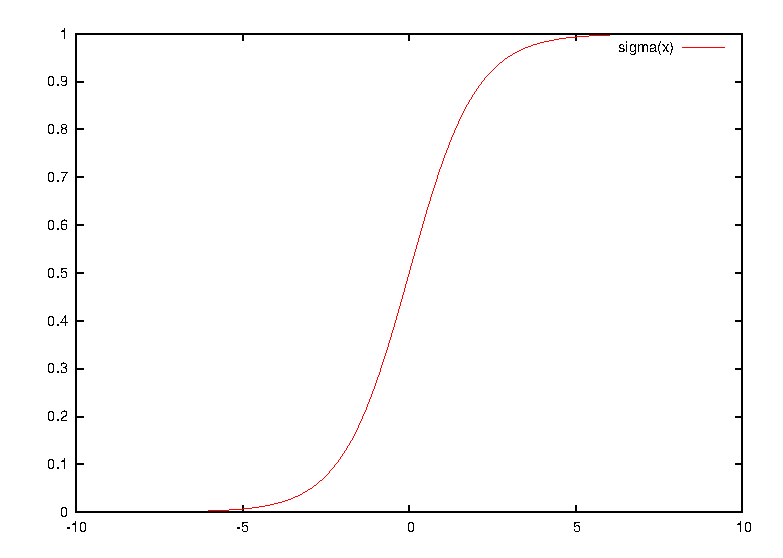
\includegraphics[scale=0.5]{sig}
\par\end{centering}
\caption{An example plot of the sigmoid function.\protect\label{fig:sigPlot}}

\end{figure}
As it is clearly shown in this figure, the sigmoid function very quickly
takes on the value 1 as x goes towards infinity and very quickly takes
on the value 0 as x goes towards minus infinity. This behavior has
the direct result that the function loses its generalization capabilities
very quickly and these are limited to a small range of values. In
order to measure this effect, the function $B\left(N\left(\overrightarrow{x},\overrightarrow{w}\right),a\right)$
is introduced and it is shown in Algorithm \ref{alg:CalculationBound}.
The quantity $a$ is used as a threshold beyond which the artificial
neural network loses its generalization capabilities.

{\bfseries{}
\begin{algorithm}[H]
\textbf{\caption{Calculating the quantity $B(N\left(\protect\overrightarrow{x},\protect\overrightarrow{w}\right),a)$
with $a>0$ for a a provided neural network $N(x,w).$\protect\label{alg:CalculationBound}}
}
\begin{enumerate}
\item \textbf{Function} $B(N\left(\overrightarrow{x},\overrightarrow{w}\right),a)$
\item \textbf{Inputs}: The neural network $N\left(\overrightarrow{x},\overrightarrow{w}\right)$
and the bound factor $a>0$.
\item \textbf{Set $k=0$}
\item \textbf{For $i=1..H$ Do}
\begin{enumerate}
\item \textbf{For $j=1..M$ Do}
\begin{enumerate}
\item Set $v=\sum_{k=1}^{d}\left(w_{(d+2)i-(d+i)+k}x_{jk}\right)+w_{(d+2)i}$
\item \textbf{If $\left|v\right|>a$ then $k=k+1$}
\end{enumerate}
\item \textbf{EndFor}
\end{enumerate}
\item \textbf{EndFor}
\item \textbf{Return $\frac{k}{H\star M}$}
\item \textbf{End Function}
\end{enumerate}
\end{algorithm}
}The steps of the used algorithm are outlined below:
\begin{enumerate}
\item \textbf{Initialization step}.
\begin{enumerate}
\item \textbf{Set} $N_{g}$ as the maximum number of allowed generations.
\item \textbf{Set} $N_{c}$ the number of used chromosomes. Each chromosome
is considered as a vector of $n=\left(d+2\right)H$ double precision
values. The value $d$ is used to represent the dimension of the input
pattern and the constant $H$ defines the number of the nodes of the
neural network. Every value in the chromosomes is initialized randomly
in the range $\left[-I_{0},I_{0}\right],I_{0}>0$.
\item \textbf{Set} $p_{s}$ the selection rate, where $p_{s}\le1$.
\item \textbf{Set} $p_{m}$ the mutation rate, where $p_{m}\le1$.
\item \textbf{Set} $k=0$ the generation counter.
\end{enumerate}
\item \textbf{Fitness calculation step}.
\begin{enumerate}
\item \textbf{For} $i=1,\ldots,N_{c}$ \textbf{do}
\begin{enumerate}
\item \textbf{Create} the neural network $N_{i}\left(\overrightarrow{x},\overrightarrow{g_{i}}\right)$
for the chromosome $\overrightarrow{g_{i}}$.
\item \textbf{Set} $E_{i}=\sum_{j=1}^{M}\left(N\left(\overrightarrow{x_{j}},\overrightarrow{g_{i}}\right)-y_{j}\right)^{2}$
\item \textbf{Set} $b_{i}=B(N\left(\overrightarrow{x},\overrightarrow{g_{i}}\right),a)$
using the function of Algorithm \ref{alg:CalculationBound}.
\item \textbf{Set} $f_{i}=E\left(N\left(\overrightarrow{x},\overrightarrow{g_{i}}\right)\right)\times\left(1+\lambda b_{i}^{2}\right)$
as value for the fitness of chromosome $g_{i}$, with $\lambda>1$. 
\end{enumerate}
\item \textbf{End For}
\end{enumerate}
\item \textbf{Application of genetic operations}.
\begin{enumerate}
\item \textbf{Copy} the best $\left(1-p_{s}\right)\times N_{c}$ chromosomes
of the current population intact to the next generation. The remaining
of chromosomes will be replaced by new chromosomes produced during
crossover and mutation.
\item \textbf{Perform }the crossover procedure. For each new element, two
parents $z=\left(z_{1},z_{2},...,z_{n}\right),\ \ w=\left(w_{1},w_{2},...,w_{n}\right)$
are selected from the current population using using tournament selection.
After the selection of the parents, the new offsprings $\tilde{z}$
and $\tilde{w}$ are formed using the following:
\begin{eqnarray}
\tilde{z_{i}} & = & r_{i}z_{i}+\left(1-r_{i}\right)w_{i}\nonumber \\
\tilde{w_{i}} & = & r_{i}w_{i}+\left(1-r_{i}\right)z_{i}\label{eq:crossover_ali}
\end{eqnarray}
where $r_{i}$ are random numbers in $[-0.5,1.5]$ \citep{weight_gpu2}. 
\item \textbf{Perform} the mutation procedure, as proposed in \citep{kaelo}:
For every chromosome and each element select a random number $r\in[0,1]$.
If $r\le p_{m}$ alter the corresponding element $g_{ij}$ as
\begin{equation}
g_{ij}=\left\{ \begin{array}{cc}
g_{ij}+\Delta\left(\mbox{t},b_{g,i}-g_{ij}\right) & t=0\\
g_{ij}-\Delta\left(\mbox{t},g_{ij}-a_{g,i}\right) & t=1
\end{array}\right.\label{eq:ali_mutation}
\end{equation}
The number $t$ is a random number that can be 0 or 1 and the function
$\Delta(\mbox{t},y)$ is calculated as:
\begin{equation}
\Delta(t,y)=y\left(1-\omega^{\left(1-\frac{t}{N_{t}}\right)z}\right)\label{eq:delta_equation}
\end{equation}
where $\omega\in[0,1]$ is a random number and $z$ is parameter defined
from the user. 
\end{enumerate}
\item \textbf{Termination check step}.
\begin{enumerate}
\item \textbf{Set} $k=k+1$
\item \textbf{If} $k<N_{g}$ go to Fitness Calculation step.
\end{enumerate}
\item \textbf{Final Step}.
\begin{enumerate}
\item \textbf{Get} the chromosome $g^{*}$ having the lowest fitness value
in the population.
\item \textbf{Produce }the vectors $L^{*}$and $R^{*}$ using the following:
\[
\begin{array}{ccc}
L_{i}^{*} & = & -f\left|g_{i}^{*}\right|,\ i=1,\ldots,n\\
R_{i}^{*} & = & f\left|g_{i}^{*}\right|,\ i=1,\ldots,n
\end{array}
\]
where $f>1$. These vectors will be used in the following phase of
the proposed algorithm.
\end{enumerate}
\end{enumerate}

\subsection{The algorithm of the second stage }

In the second phase of the current work, a bound method is applied
using the vectors $L^{*}$ and $R^{*}$ of the previous stage, to
discover the optimal bound for the parameters of the network. During
this phase, a modified genetic algorithm is incorporated, where the
chromosomes are defined as interval sets $\left[\overrightarrow{L_{k}},\overrightarrow{R_{k}}\right]$.
Also, the fitness value for each chromosome is considered as an interval
$f=\left[f_{1},f_{2}\right].$ The function $D(a,b)$ is introduced
here for the comparison of two intervals $a=\left[a_{1},a_{2}\right]$
and $b=\left[b_{1},b_{2}\right].$ This function is defined as:
\begin{equation}
D(a,b)=\begin{cases}
\mbox{TRUE}, & a_{1}<b_{1},\mbox{OR\ \ensuremath{\left(a_{1}=b_{1}\ \mbox{AND}\ a_{2}<b_{2}\right)}}\\
\mbox{FALSE}, & \mbox{\mbox{OTHERWISE}}
\end{cases}\label{eq:eqD}
\end{equation}
A modified genetic algorithm is incorporated here to locate the most
promising interval for the weights of the neural network. This procedure
uses the vectors $L^{*}$ and $R^{*}$ of the previous algorithm.
Each chromosome is considered as a set of intervals, which is initialized
randomly inside\textbf{ }the vectors $L^{*}$ and $R^{*}$. The steps
of the algorithm for the second phase are presented below:
\begin{enumerate}
\item \textbf{Initialization step}.
\begin{enumerate}
\item \textbf{Set} as $N_{g}$ the maximum number of allowed generations
and as $N_{c}$ the total number of chromosomes.
\item \textbf{Set} as $p_{s}$ the selection rate and as $p_{m}$ the mutation
rate.
\item \textbf{Initialize} every chromosomes$g_{i}=$$\left[\overrightarrow{L_{i}},\overrightarrow{R_{i}}\right],\ i=1,\ldots,N_{c}$
randomly inside the produced vectors $L^{*}$and $R^{*}$ from the
previous phase.
\item \textbf{Set} as $N_{s}$ the number of samples used in the fitness
calculation step.
\item \textbf{Set} $k=0$, the generation counter.
\end{enumerate}
\item \textbf{Fitness calculation step}.
\begin{enumerate}
\item \textbf{For} $i=1,\ldots,N_{c}$ \textbf{do}
\begin{enumerate}
\item \textbf{Calculate} the fitness $f_{i}$ of each chromosome $g_{i}$
using the procedure provided in Algorithm \ref{alg:fitnessCalculation}.
\end{enumerate}
\item \textbf{End For}
\end{enumerate}
\item \textbf{Application of genetic operators}.
\begin{enumerate}
\item Selection procedure. Copy the best $\left(1-p_{s}\right)\times N_{c}$
chromosomes to the next generation without changes. The remaining
ones will be replaced by offsprings created using the crossover and
the mutation procedure. The sorting is performed using the operator
$D(a,b)$ for the fitness values.
\item Crossover procedure. Perform the crossover procedure, where for every
couple $\left(\widetilde{z},\widetilde{w}\right)$ of produced chromosomes,
two parents $\left(z,w\right)$will be chosen using tournament selection.
The new chromosomes will be produced using the one - point crossover
method, graphically presented in Figure \ref{fig:onePoint}.
\item Mutation procedure. For each element of each chromosome a random number
$r\in[0,1]$ is drawn. The corresponding element is altered randomly
when $r\le p_{m}$.
\end{enumerate}
\item \textbf{Termination check step}.
\begin{enumerate}
\item \textbf{Set} $k=k+1$
\item \textbf{If} $k<N_{g}$ go to Fitness calculation step.
\end{enumerate}
\item \textbf{Final step}.
\begin{enumerate}
\item \textbf{Obtain} the best chromosome from the population $g^{*}$
\item \textbf{Produce} the corresponding set of intervals $\left[\overrightarrow{L^{*}},\overrightarrow{R^{*}}\right]$
\end{enumerate}
\end{enumerate}
\begin{algorithm}[H]
\caption{Fitness calculation function. \protect\label{alg:fitnessCalculation}}

\begin{enumerate}
\item \textbf{function }fitness$\left(g,N_{s}\right)$
\item \textbf{Input}: The chromosome $g=\left[\overrightarrow{L_{g}},\overrightarrow{R_{g}}\right]$
and the number of random samples $N_{s}$.
\item \textbf{Draw} $N_{s}$ random samples in $g$ and create the set $S_{a}=\left\{ \overrightarrow{s_{1}},\overrightarrow{s_{2},}\ldots,\overrightarrow{s_{N_{s}}}\right\} $.
\item \textbf{Set} $f_{\mbox{min}}=\infty$
\item \textbf{Set} $f_{\max}=-\infty$
\item \textbf{For} $i=1,\ldots,N_{s}$ \textbf{do}
\begin{enumerate}
\item \textbf{Set} $E_{i}=\sum_{j=1}^{M}\left(N\left(\overrightarrow{x_{j}},\overrightarrow{s_{i}}\right)-y_{j}\right)^{2}$
\item \textbf{If} $E_{i}<f_{\mbox{min}}$ set $f_{\mbox{min}}=E_{i}$
\item \textbf{If} $E_{i}>f_{\mbox{max}}$ set $f_{\mbox{max}}=E_{i}$
\end{enumerate}
\item \textbf{End For}
\item \textbf{Return} as fitness value the quantity $f_{g}=\left[f_{\mbox{min}},f_{\mbox{max}}\right]$
\item \textbf{End Function}
\end{enumerate}
\end{algorithm}

\begin{figure}[H]
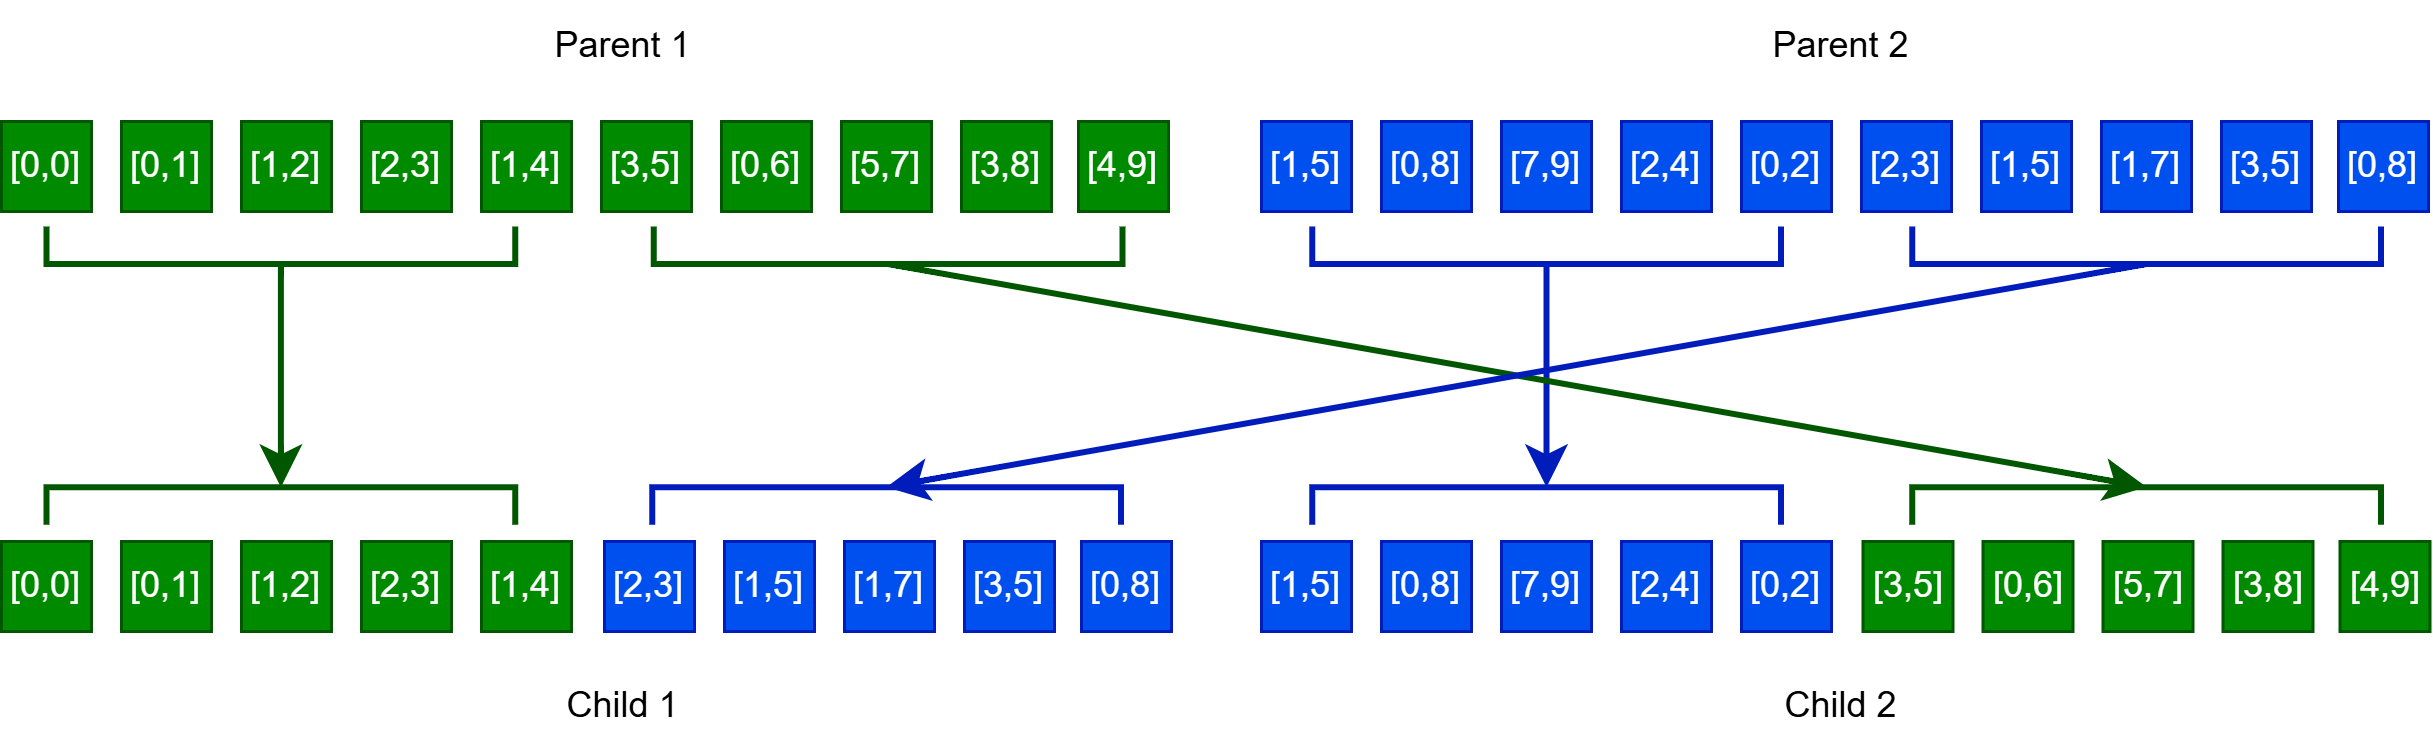
\includegraphics[scale=0.5]{crossover}

\caption{An example of the one - point crossover procedure.\protect\label{fig:onePoint}}

\end{figure}


\subsection{The final training algorithm}

During the final step of the proposed method, a genetic algorithm
is incorporated to train the artificial neural network inside the
bounds $\left[\overrightarrow{L^{*}},\overrightarrow{R^{*}}\right]$
produced in the final step of the previous phase of the method. The
main steps of this algorithm are listed below:
\begin{enumerate}
\item \textbf{Initialization step}.
\begin{enumerate}
\item \textbf{Set} as $N_{g}$ the maximum number of allowed generations
and as $N_{c}$ the total number of chromosomes.
\item \textbf{Set} as $p_{s}$ the selection rate and as $p_{m}$ the mutation
rate.
\item \textbf{Initialize} randomly the chromosomes $g_{i},\ i=1,\ldots,N_{c}$
as random vectors with $n=(d+2)H$ elements inside the bounds $\left[\overrightarrow{L^{*}},\overrightarrow{R^{*}}\right]$.
\item \textbf{Set} $k=0$, the generation counter.
\end{enumerate}
\item \textbf{Fitness calculation step}.
\begin{enumerate}
\item \textbf{For} $i=1,\ldots,N_{c}$ \textbf{do}
\begin{enumerate}
\item \textbf{Create} the neural network $N_{i}\left(\overrightarrow{x},\overrightarrow{g_{i}}\right)$
for the chromosome $\overrightarrow{g_{i}}$.
\item \textbf{Calculate} the associated fitness value $f_{i}$ as $f_{i}=\sum_{j=1}^{M}\left(N\left(\overrightarrow{x_{j}},\overrightarrow{g_{i}}\right)-y_{j}\right)^{2}$
\end{enumerate}
\item \textbf{End For}
\end{enumerate}
\item \textbf{Incorporation of genetic operators.} Apply the same genetic
operators as in the first phase of the proposed algorithm, described
in subsection \ref{subsec:firstPhase}. 
\item \textbf{Termination check step}.
\begin{enumerate}
\item \textbf{Set} $k=k+1$
\item \textbf{If} $k<N_{g}$ go to Fitness Calculation step of the current
algorithm.
\end{enumerate}
\item \textbf{Testing step}.
\begin{enumerate}
\item \textbf{Obtain} the chromosome with the lowest fitness value in the
population and denote it as $g^{*}$.
\item \textbf{Produce} the associated neural network $N\left(\overrightarrow{x},\overrightarrow{g^{*}}\right)$
\item \textbf{Apply} a local search procedure to the error function for
this network. The local search procedure used was a BFGS method of
Powell \citep{powell}.
\item \textbf{Apply} the neural network on the associated test set of the
problem to obtain the test error.
\end{enumerate}
\end{enumerate}

\section{Results\protect\label{sec:Results}}

The validation of the proposed method was performed using a wide series
of classification and regression datasets, available from various
sources from the Internet. These datasets were downloaded from:
\begin{enumerate}
\item The UCI database, \url{https://archive.ics.uci.edu/}(accessed on
30 April 2025)\citep{uci}
\item The Keel website, \url{https://sci2s.ugr.es/keel/datasets.php}(accessed
on 30 April 2025)\citep{Keel}.
\item The Statlib URL \url{https://lib.stat.cmu.edu/datasets/index}(accessed
on 30 April 2025). 
\end{enumerate}

\subsection{Experimental datasets }

The following datasets were utilized in the conducted experiments:
\begin{enumerate}
\item \textbf{Appendictis} which is a medical dataset \citep{appendicitis}. 
\item \textbf{Alcohol}, which is dataset regarding alcohol consumption \citep{alcohol}. 
\item \textbf{Australian}, which is a dataset produced from various bank
transactions \citep{australian}.
\item \textbf{Balance} dataset \citep{balance}, produced from various psychological
experiments.
\item \textbf{Cleveland}, a medical dataset which was discussed in a series
of papers \citep{cleveland1,cleveland2}. 
\item \textbf{Circular} dataset, which is an artificial dataset.
\item \textbf{Dermatology}, a medical dataset for dermatology problems \citep{dermatology}.
\item The \textbf{Hayes-roth} dataset, which was initially suggested in
\citep{hayes-roth}.
\item \textbf{Heart}, which is a dataset related to heart diseases \citep{heart}.
\item \textbf{HeartAttack}, which is related to heart diseases
\item \textbf{Housevotes}, a dataset which contains data from the Congressional
voting in USA \citep{housevotes}.
\item \textbf{Ionosphere}, which is related to measurements derived from
the ionosphere \citep{ion1,ion2}.
\item \textbf{Liverdisorder}, a medical dataset \citep{liver,liver1}.
\item The \textbf{Lymography} dataset \citep{lymography}.
\item \textbf{Mammographic}, which is related to the presence of breast
cancer \citep{mammographic}.
\item \textbf{Parkinsons}, which is a medical dataset used for the detection
of Parkinson's disease \citep{parkinsons1,parkinsons2}.
\item \textbf{Pima}, which is related to the presence of diabetes\citep{pima}.
\item \textbf{Popfailures}, a dataset related to experiments regarding climate
\citep{popfailures}.
\item \textbf{Regions2}, a medical dataset applied to liver problems \citep{regions2}.
\item \textbf{Saheart}, which is a medical dataset concerning heart diseases\citep{saheart}.
\item \textbf{Segment} dataset \citep{segment}.
\item The Sonar dataset, related to sonar signals \citep{sonar}.
\item \textbf{Statheart}, a medical dataset related to heart diseases.
\item \textbf{Spiral}, which was created artificially and contains two distinct
classes.
\item \textbf{Student}, which is a dataset regarding experiments in schools
\citep{student}.
\item \textbf{Transfusion}, which is also a dataset used for medical purposes
\citep{transfusion}.
\item \textbf{Wdbc}, which is used for the detection of breast cancer \citep{wdbc1,wdbc2}.
\item \textbf{Wine}, a dataset used to detect the quality of wines \citep{wine1,wine2}.
\item \textbf{EEG}, which is a dataset regarding EEG recordings \citep{eeg1,eeg2}
and from this dataset the following cases were used: Z\_F\_S, ZO\_NF\_S,
ZONF\_S and Z\_O\_N\_F\_S.
\item \textbf{Zoo}, which is a dataset regarding animal classification \citep{zoo}
.
\end{enumerate}
Moreover a series of regression datasets was adopted in the performed
experiments. The list with the regression datasets has as follows:
\begin{enumerate}
\item \textbf{Abalone}, which is a dataset for the detection of the age
of abalones \citep{abalone}.
\item \textbf{Airfoil}, founded in NASA \citep{airfoil}.
\item \textbf{Auto}, a dataset used to predict the fuel consumption in cars.
\item \textbf{BK}, which is used to predict the points scored in basketball
games. 
\item \textbf{BL}, a dataset that contains measurements from electricity
experiments.
\item \textbf{Baseball}, which is a dataset used to predict the income of
baseball players.
\item \textbf{Concrete}, which is a civil engineering dataset \citep{concrete}.
\item \textbf{DEE}, a dataset that is used to predict the price of electricity.
\item \textbf{Friedman}, which is an artificial dataset\citep{friedman}.
\item \textbf{FY, }which is a dataset regarding the longevity of fruit flies. 
\item \textbf{HO}, a dataset located in the STATLIB repository.
\item \textbf{Housing}, regarding the price of houses \citep{housing}.
\item \textbf{Laser}, which is used in physics experiments.
\item The \textbf{MB} dataset, originated in the Smoothing Methods in Statistics.
\item The\textbf{ NT} dataset\citep{ntdataset}.
\item \textbf{Mortgage}, a dataset that contains data from the economy of
USA.
\item \textbf{PL} dataset, located in the STALIB repository.
\item \textbf{Plastic}, a dataset regarding problems occurred with the pressure
on plastics.
\item The \textbf{PY} dataset \citep{pydataset}.
\item \textbf{Quake}, a dataset regarding the measurements of earthquakes.
\item \textbf{SN}, a dataset related to trellising and pruning.
\item \textbf{Stock}, which related to the prices of stocks.
\item \textbf{Treasury}, a dataset that contains measurements from the economy
of USA.
\end{enumerate}

\subsection{Experimental results}

The software used in the experiment was coded in C++ with the assistance
of the freely available Optimus environment \citep{optimus}. Each
experiment was conducted 30 times and in every execution a different
seed for the random generator was used. For the validation of the
experimental results, the ten - fold cross validation technique was
used. The average classification error, as measured in the corresponding
test set was reported for the classification datasets. The classification
error is computed using the following formula:
\begin{equation}
E_{C}\left(N\left(\overrightarrow{x},\overrightarrow{w}\right)\right)=100\times\frac{\sum_{i=1}^{N}\left(\mbox{class}\left(N\left(\overrightarrow{x_{i}},\overrightarrow{w}\right)\right)-y_{i}\right)}{N}
\end{equation}
For the calculation of this error, the test set $T$ is a set $T=\left(x_{i},y_{i}\right),\ i=1,\ldots,N$
is used. Similarly, the average regression error is reported for the
regression datasets and it is calculated as follows:
\begin{equation}
E_{R}\left(N\left(\overrightarrow{x},\overrightarrow{w}\right)\right)=\frac{\sum_{i=1}^{N}\left(N\left(\overrightarrow{x_{i}},\overrightarrow{w}\right)-y_{i}\right)^{2}}{N}
\end{equation}

Table \ref{tab:expValues} contains the values used for the experimental
parameters of the proposed method. The results obtained for the classification
datasets are depicted in Table \ref{tab:experClass} and for the regression
datasets in Table \ref{tab:experRegression}. The following notations
were used for the experimental tables:
\begin{enumerate}
\item The column DATASET is used to denote the name of the dataset.
\item The column BFGS represents the results obtained by the training of
a neural network with $H=10$ processing nodes using the BFGS optimization
method \citep{powell} .
\item The column ADAM is used to denote the training of a neural network
with $H=10$ processing nodes using the ADAM optimization method \citep{nn_adam}.
\item The column NEAT represents the incorporation of the NEAT method (NeuroEvolution
of Augmenting Topologies ) \citep{neat}.
\item The column RBF is used to denote the usage of a Radial Basis Function
(RBF) network \citep{rbf1,rbf2} with 10 processing nodes.
\item The column GENETIC denotes the usage of a genetic algorithm to train
a neural network with $H=10$ processing nodes.
\item The column PROPOSED denotes experimental results of the proposed method.
\item The row AVERAGE represents the average classification or regression
error for all datasets.
\end{enumerate}
\begin{table}[H]
\caption{The values for the parameters of the proposed method.\protect\label{tab:expValues}}

\centering{}%
\begin{tabular}{|c|c|c|}
\hline 
PARAMETER & MEANING & VALUE\tabularnewline
\hline 
\hline 
$N_{c}$ & Chromosomes & 500\tabularnewline
\hline 
$N_{g}$ & Maximum number of generations & 200\tabularnewline
\hline 
$p_{S}$ & Selection rate & 0.1\tabularnewline
\hline 
$p_{M}$ & Mutation rate & 0.05\tabularnewline
\hline 
$H$ & Number of nodes & 10\tabularnewline
\hline 
$I_{0}$ & Initialization factor & 10.0\tabularnewline
\hline 
$a$ & Bounding factor & 10.0\tabularnewline
\hline 
$f$ & Scale factor for the margins & 2.0\tabularnewline
\hline 
$\lambda$ & Value used for penalties & 100.0\tabularnewline
\hline 
\end{tabular}
\end{table}

The Table \ref{tab:experClass} presented shows the error rates resulting
from the incorporation of the mentioned machine learning models on
the used classification datasets. The columns refer to the models
(BFGS, ADAM, NEAT, RBF, GENETIC, PROPOSED), while the rows correspond
to the datasets. From the analysis of the data, it is observed that
the PROPOSED model exhibits the lowest error rates in many datasets,
such as \textquotedbl HouseVotes\textquotedbl{} (3.05\%), \textquotedbl Dermatology\textquotedbl{}
(5.97\%), and \textquotedbl ZONF\_S\textquotedbl{} (2.35\%). Furthermore,
it has the lowest average error rate (19.49\%) when a comparison is
made against to the other models, indicating overall superior performance.
The NEAT model shows the highest error rates in several cases, such
as \textquotedbl Cleveland\textquotedbl{} (77.55\%) and \textquotedbl Segment\textquotedbl{}
(68.97\%), while ADAM and BFGS exhibit high errors in datasets like
\textquotedbl Z\_F\_S\textquotedbl{} (47.81\% and 39.37\%, respectively).
However, ADAM has a slightly better average error rate (33.73\%) compared
to other traditional models like BFGS (33.50\%) and NEAT (32.77\%).
The GENETIC model, although competitive in some datasets like \textquotedbl Hayes
Roth\textquotedbl{} (56.18\%) and \textquotedbl Z\_O\_N\_F\_S\textquotedbl{}
(64.81\%), has a higher average error rate (25.68\%) compared to RBF
(28.54\%). RBF, though not the best in terms of accuracy, demonstrates
balanced performance in many cases, with low error rates in datasets
such as \textquotedbl Popfailures\textquotedbl{} (7.04\%) and \textquotedbl HouseVotes\textquotedbl{}
(6.13\%). Overall, the PROPOSED model stands out as the most effective,
with the lowest average error rates and exceptional performance across
multiple dataset categories, making it the preferred choice for classification
tasks.
\begin{table}[H]
\caption{Experimental results using the incorporated machine learning methods
on the classification datasets. The numbers in cells represent average
classification error for the test set.\protect\label{tab:experClass}}

\centering{}%
\begin{tabular}{|c|c|c|c|c|c|c|}
\hline 
\textbf{DATASET} & \textbf{BFGS} & \textbf{ADAM} & \textbf{NEAT} & \textbf{RBF} & \textbf{GENETIC} & \textbf{PROPOSED}\tabularnewline
\hline 
\hline 
Alcohol & 41.50\% & 57.78\% & 66.80\% & 49.38\% & 39.57\% & 26.24\%\tabularnewline
\hline 
Appendicitis & 18.00\% & 16.50\% & 17.20\% & 12.23\% & 18.10\% & 14.90\%\tabularnewline
\hline 
Australian & 38.13\% & 35.65\% & 31.98\% & 34.89\% & 32.21\% & 31.64\%\tabularnewline
\hline 
Balance & 8.64\% & 7.87\% & 23.14\% & 33.42\% & 8.97\% & 7.80\%\tabularnewline
\hline 
Cleveland & 77.55\% & 67.55\% & 53.44\% & 67.10\% & 51.60\% & 47.51\%\tabularnewline
\hline 
Circular & 6.08\% & 19.95\% & 35.18\% & 5.98\% & 5.99\% & 5.42\%\tabularnewline
\hline 
Dermatology & 52.92\% & 26.14\% & 32.43\% & 62.34\% & 30.58\% & 5.97\%\tabularnewline
\hline 
Hayes Roth & 37.33\% & 59.70\% & 50.15\% & 64.36\% & 56.18\% & 39.28\%\tabularnewline
\hline 
Heart & 39.44\% & 38.53\% & 39.27\% & 31.20\% & 28.34\% & 16.85\%\tabularnewline
\hline 
HeartAttack & 46.67\% & 45.55\% & 32.34\% & 29.00\% & 29.03\% & 23.77\%\tabularnewline
\hline 
HouseVotes & 7.13\% & 7.48\% & 10.89\% & 6.13\% & 6.62\% & 3.05\%\tabularnewline
\hline 
Ionosphere & 15.29\% & 16.64\% & 19.67\% & 16.22\% & 15.14\% & 8.75\%\tabularnewline
\hline 
Liverdisorder & 42.59\% & 41.53\% & 30.67\% & 30.84\% & 31.11\% & 29.53\%\tabularnewline
\hline 
Lymography & 35.43\% & 29.26\% & 33.70\% & 25.50\% & 28.42\% & 17.17\%\tabularnewline
\hline 
Mammographic & 17.24\% & 46.25\% & 22.85\% & 21.38\% & 19.88\% & 16.45\%\tabularnewline
\hline 
Parkinsons & 27.58\% & 24.06\% & 18.56\% & 17.41\% & 18.05\% & 17.46\%\tabularnewline
\hline 
Pima & 35.59\% & 34.85\% & 34.51\% & 25.78\% & 32.19\% & 27.25\%\tabularnewline
\hline 
Popfailures & 5.24\% & 5.18\% & 7.05\% & 7.04\% & 5.94\% & 4.66\%\tabularnewline
\hline 
Regions2 & 36.28\% & 29.85\% & 33.23\% & 38.29\% & 29.39\% & 25.88\%\tabularnewline
\hline 
Saheart & 37.48\% & 34.04\% & 34.51\% & 32.19\% & 34.86\% & 31.59\%\tabularnewline
\hline 
Segment & 68.97\% & 49.75\% & 66.72\% & 59.68\% & 57.72\% & 42.43\%\tabularnewline
\hline 
Sonar & 25.85\% & 30.33\% & 34.10\% & 27.90\% & 22.40\% & 19.30\%\tabularnewline
\hline 
Spiral & 47.99\% & 48.90\% & 50.22\% & 44.87\% & 48.66\% & 44.67\%\tabularnewline
\hline 
Statheart & 39.65\% & 44.04\% & 44.36\% & 31.36\% & 27.25\% & 18.90\%\tabularnewline
\hline 
Student & 7.14\% & 5.13\% & 10.20\% & 5.49\% & 5.61\% & 4.33\%\tabularnewline
\hline 
Transfusion & 25.84\% & 25.68\% & 24.87\% & 26.41\% & 24.87\% & 23.60\%\tabularnewline
\hline 
Wdbc & 29.91\% & 35.35\% & 12.88\% & 7.27\% & 8.56\% & 8.69\%\tabularnewline
\hline 
Wine & 59.71\% & 29.40\% & 25.43\% & 31.41\% & 19.20\% & 7.27\%\tabularnewline
\hline 
Z\_F\_S & 39.37\% & 47.81\% & 38.41\% & 13.16\% & 10.73\% & 5.33\%\tabularnewline
\hline 
Z\_O\_N\_F\_S & 65.67\% & 78.79\% & 77.08\% & 48.70\% & 64.81\% & 53.15\%\tabularnewline
\hline 
ZO\_NF\_S & 43.04\% & 47.43\% & 43.75\% & 9.02\% & 21.54\% & 5.82\%\tabularnewline
\hline 
ZONF\_S & 15.62\% & 11.99\% & 5.44\% & 4.03\% & 4.36\% & 2.35\%\tabularnewline
\hline 
ZOO & 10.70\% & 14.13\% & 20.27\% & 21.93\% & 9.50\% & 6.07\%\tabularnewline
\hline 
\textbf{AVERAGE} & \textbf{33.50\%} & \textbf{33.73\%} & \textbf{32.77\%} & \textbf{28.54\%} & \textbf{25.68\%} & \textbf{19.49\%}\tabularnewline
\hline 
\end{tabular}
\end{table}

Executions were carried out using scripts in the R language, based
on the experimental measurement tables, to determine the significance
levels of the experiments using the critical parameter p. In Figure
\ref{fig:stat1}, the significance levels are presented, referring
to classification datasets and comparing the performance of the PROPOSED
model with various machine learning models. The comparisons include
the following cases: PROPOSED vs BFGS with p={*}{*}{*}{*} (Very extremely
significant), \textbf{(OK)}PROPOSED vs ADAM with p={*}{*}{*}{*}, PROPOSED
vs NEAT with p={*}{*}{*}{*}, PROPOSED vs RBF with p={*}{*}{*}{*},
and PROPOSED vs GENETIC with p={*}{*}{*}{*}. The results provide a
clear assessment of the statistical significance of the differences
in performance between the PROPOSED model and the other models. The
lower the p-value, the stronger the indication that the observed difference
in performance is not due to random factors but reflects the genuine
superiority of the PROPOSED model.

\begin{figure}[H]
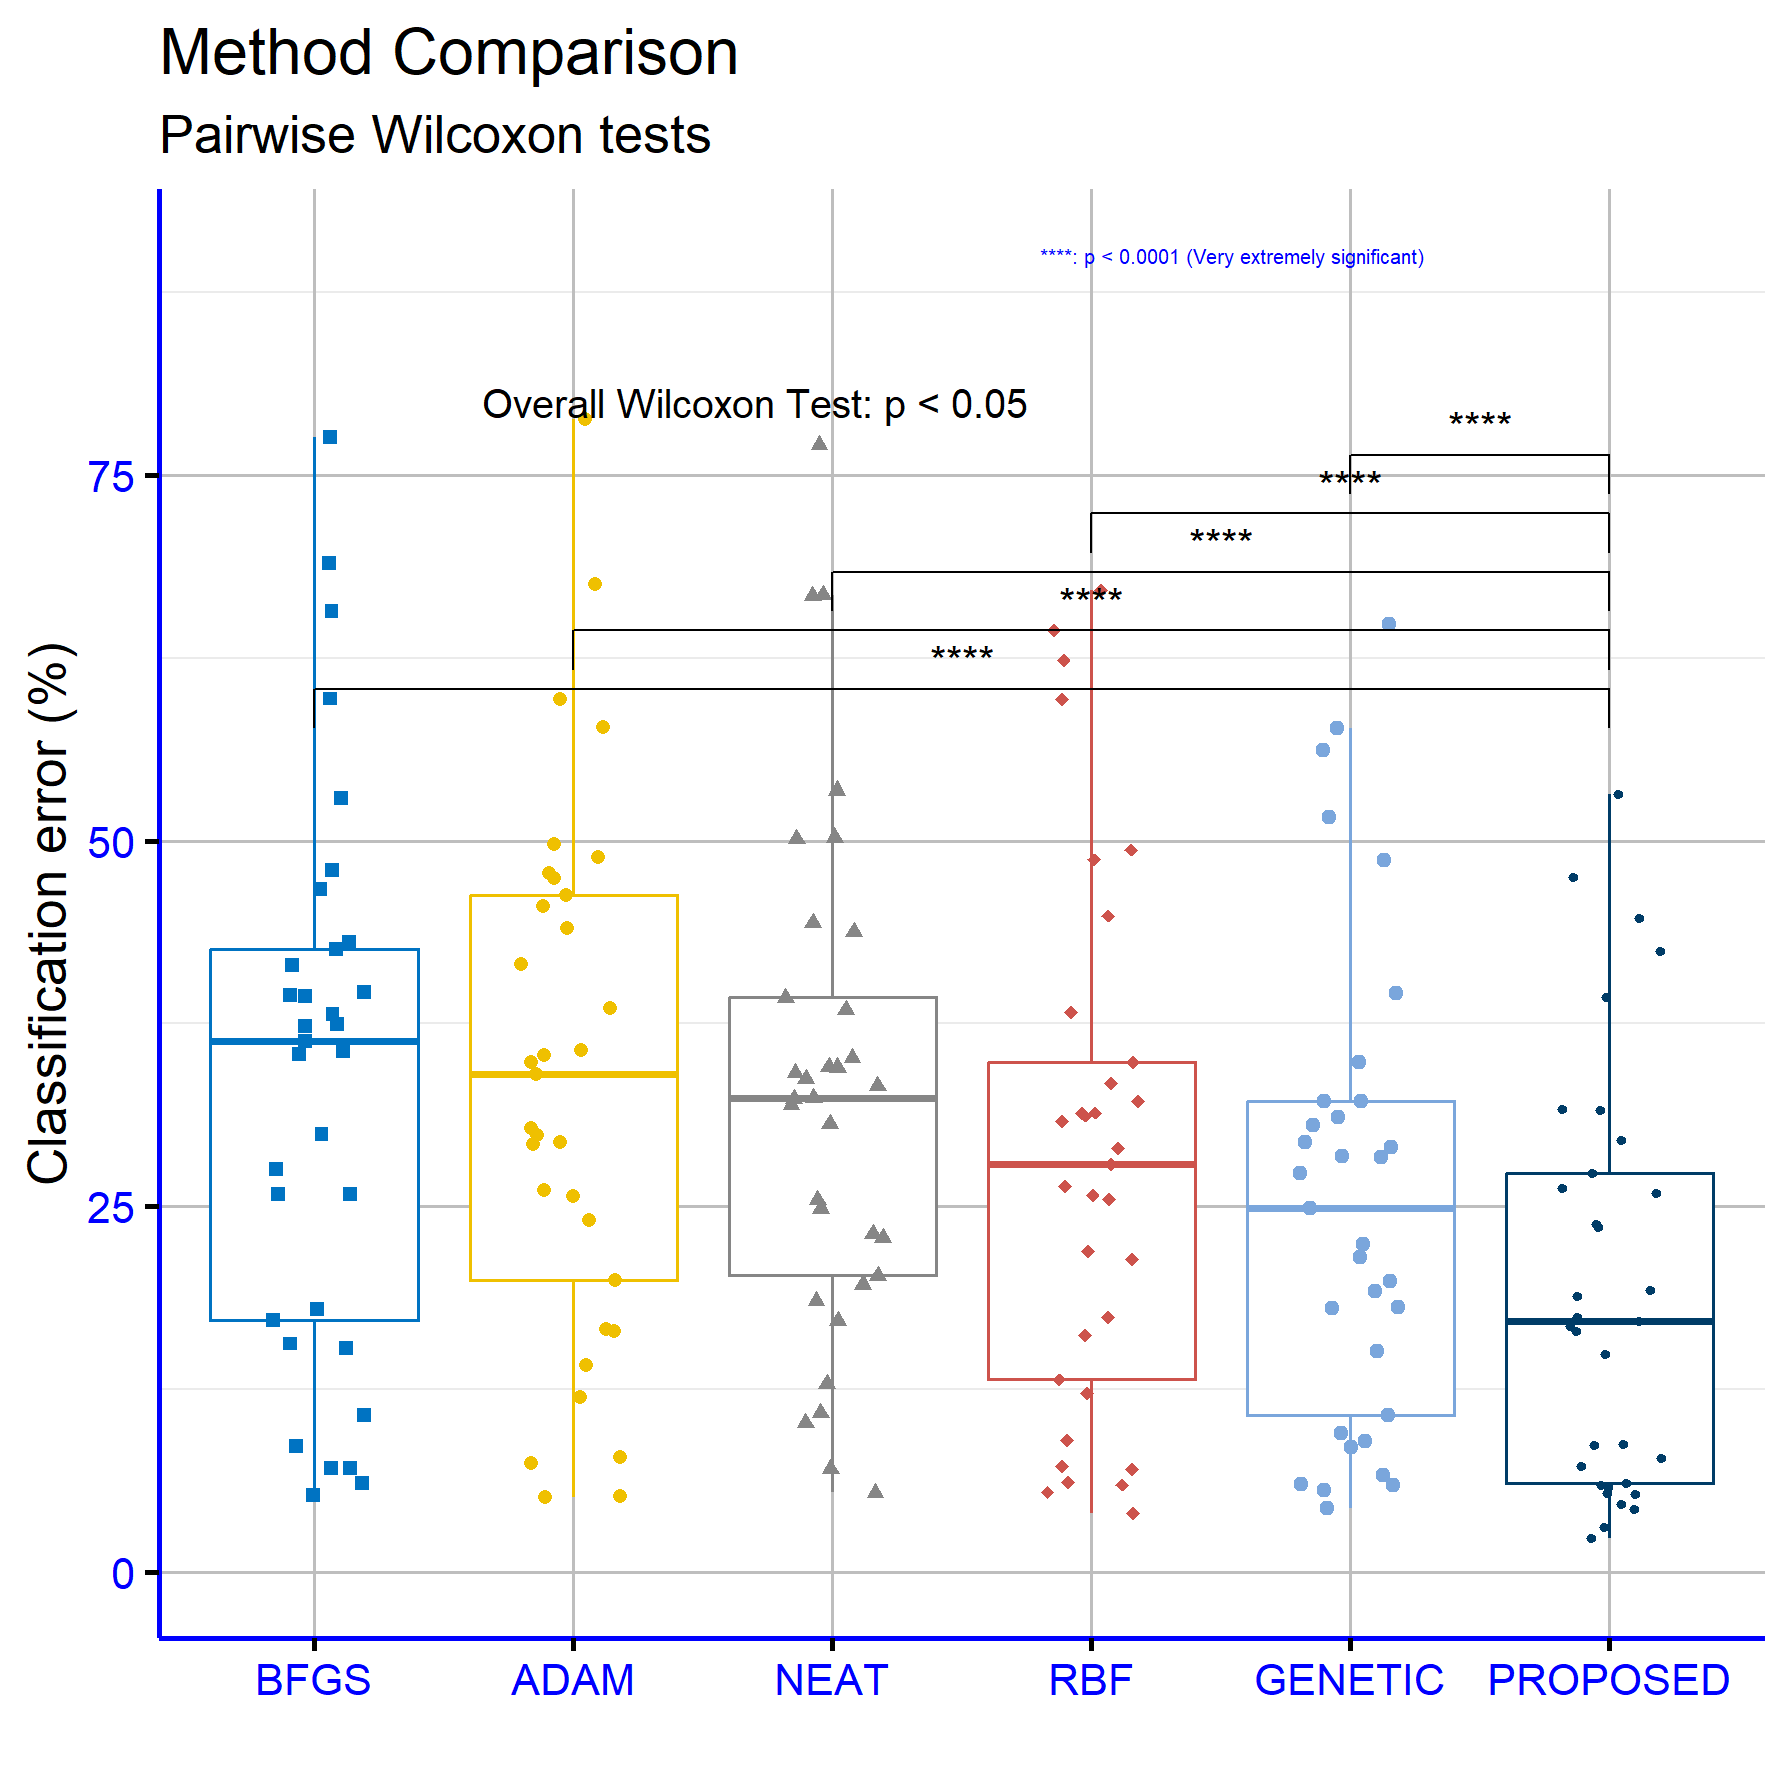
\includegraphics[scale=0.5]{stat1}

\caption{Statistical comparison for the applied machine learning methods and
the classification datasets.\protect\label{fig:stat1}}
\end{figure}

The Table \ref{tab:experRegression} presents the obtained regression
errors from the usage of different machine learning models on regression
datasets. The columns refer to the models (BFGS, ADAM, NEAT, RBF,
GENETIC, PROPOSED), while the rows correspond to the datasets. From
the analysis of the data, it is evident that the PROPOSED model managed
to achieve the lowest average error (5.33). This model exhibits exceptionally
low errors in datasets such as \textquotedbl BL\textquotedbl{} (0.001),
\textquotedbl HO\textquotedbl{} (0.012), and \textquotedbl Concrete\textquotedbl{}
(0.004). The RBF model ranks second in performance, with an average
error of 9.19, and stands out for its low values in datasets like
\textquotedbl Laser\textquotedbl{} (0.03) and \textquotedbl PY\textquotedbl{}
(0.012). The GENETIC model, with an average error of 8.1, demonstrates
competitive performance in certain datasets like \textquotedbl Plastic\textquotedbl{}
(2.79) and \textquotedbl Treasury\textquotedbl{} (2.93), but generally
falls short compared to PROPOSED and RBF. The NEAT model has a higher
average error (12.84), though it performs well in datasets such as
\textquotedbl Stock\textquotedbl{} (12.23). The ADAM and BFGS models
exhibit the highest average errors, 19.62 and 26.43 respectively,
indicating less reliable overall performance. However, ADAM performs
well in datasets like \textquotedbl BK\textquotedbl{} (0.03) and
\textquotedbl FY\textquotedbl{} (0.038), while BFGS achieves good
values in specific datasets like \textquotedbl Airfoil\textquotedbl{}
(0.003). Overall, the PROPOSED model significantly outperforms the
others across most datasets, showcasing the best overall accuracy.
RBF and GENETIC are also reliable in specific cases, while ADAM and
BFGS, although less competitive, deliver good results in certain datasets.

\begin{table}[H]
\caption{Experimental results using the incorporated machine learning methods
on the regression datasets. The numbers in cells represent average
regression on the test set.\protect\label{tab:experRegression}}

\centering{}%
\begin{tabular}{|c|c|c|c|c|c|c|}
\hline 
\textbf{DATASET} & \textbf{BFGS} & \textbf{ADAM} & \textbf{NEAT} & \textbf{RBF} & \textbf{GENETIC} & \textbf{PROPOSED}\tabularnewline
\hline 
Abalone & 5.69 & 4.30 & 9.88 & 7.37 & 7.17 & 4.42\tabularnewline
\hline 
Airfoil & 0.003 & 0.005 & 0.067 & 0.27 & 0.003 & 0.003\tabularnewline
\hline 
Auto & 60.97 & 70.84 & 56.06 & 17.87 & 12.18 & 12.10\tabularnewline
\hline 
Baseball & 119.63 & 77.90 & 100.39 & 93.02 & 103.60 & 79.30\tabularnewline
\hline 
BK & 0.28 & 0.03 & 0.15 & 0.02 & 0.03 & 0.017\tabularnewline
\hline 
BL & 2.55 & 0.28 & 0.05 & 0.013 & 5.74 & 0.001\tabularnewline
\hline 
Concrete & 0.066 & 0.078 & 0.081 & 0.011 & 0.0099 & 0.004\tabularnewline
\hline 
Dee & 2.36 & 0.630 & 1.512 & 0.17 & 1.013 & 0.21\tabularnewline
\hline 
Housing & 97.38 & 80.20 & 56.49 & 57.68 & 43.26 & 20.74\tabularnewline
\hline 
Friedman & 1.26 & 22.90 & 19.35 & 7.23 & 1.249 & 3.569\tabularnewline
\hline 
FA & 0.426 & 0.11 & 0.19 & 0.015 & 0.025 & 0.011\tabularnewline
\hline 
FY & 0.22 & 0.038 & 0.08 & 0.041 & 0.65 & 0.038\tabularnewline
\hline 
HO & 0.62 & 0.035 & 0.169 & 0.03 & 2.78 & 0.012\tabularnewline
\hline 
Laser & 0.015 & 0.03 & 0.084 & 0.03 & 0.59 & 0.004\tabularnewline
\hline 
MB & 0.129 & 0.06 & 0.061 & 2.16 & 0.051 & 0.048\tabularnewline
\hline 
Mortgage & 8.23 & 9.24 & 14.11 & 1.45 & 2.41 & 0.85\tabularnewline
\hline 
NT & 0.129 & 0.12 & 0.33 & 8.14 & 0.006 & 0.006\tabularnewline
\hline 
PL & 0.29 & 0.117 & 0.098 & 2.12 & 0.28 & 0.022\tabularnewline
\hline 
Plastic & 20.32 & 11.71 & 20.77 & 8.62 & 2.79 & 2.20\tabularnewline
\hline 
PY & 0.578 & 0.09 & 0.075 & 0.012 & 0.564 & 0.016\tabularnewline
\hline 
Quake & 0.42 & 0.06 & 0.298 & 0.07 & 0.12 & 0.037\tabularnewline
\hline 
SN & 0.40 & 0.026 & 0.174 & 0.027 & 2.95 & 0.024\tabularnewline
\hline 
Stock & 302.43 & 180.89 & 12.23 & 12.23 & 3.88 & 3.25\tabularnewline
\hline 
Treasury & 9.91 & 11.16 & 15.52 & 2.02 & 2.93 & 1.11\tabularnewline
\hline 
\textbf{AVERAGE} & \textbf{26.43} & \textbf{19.62} & \textbf{12.84} & \textbf{9.19} & \textbf{8.10} & \textbf{5.33}\tabularnewline
\hline 
\end{tabular}
\end{table}

The figure \ref{fig:stat2} displays the results of statistical significance
tests conducted on regression datasets, aiming to evaluate the statistical
significance of performance differences between the proposed method
(PROPOSED) and other machine learning methods. The p-values obtained
from the statistical tests are extremely low, indicating strongly
statistically significant differences: for the comparison PROPOSED
vs BFGS, the p-value is {*}{*}{*}, for the comparison PROPOSED vs
ADAM, the p-value is {*}{*}{*}, for the comparison PROPOSED vs NEAT,
the p-value is {*}{*}{*}{*}, for the comparison PROPOSED vs RBF, the
p-value is {*}{*}{*} and for the comparison PROPOSED vs GENETIC, the
p-value is {*}{*}{*}. These findings demonstrate that the proposed
method does not differ randomly from the other methods but exhibits
statistically significant superiority in performance. The presence
of three or four asterisks indicates that the differences are at least
highly significant, meaning that the probability of the observed differences
being due to chance is less than 0.1\%.

\begin{figure}[H]
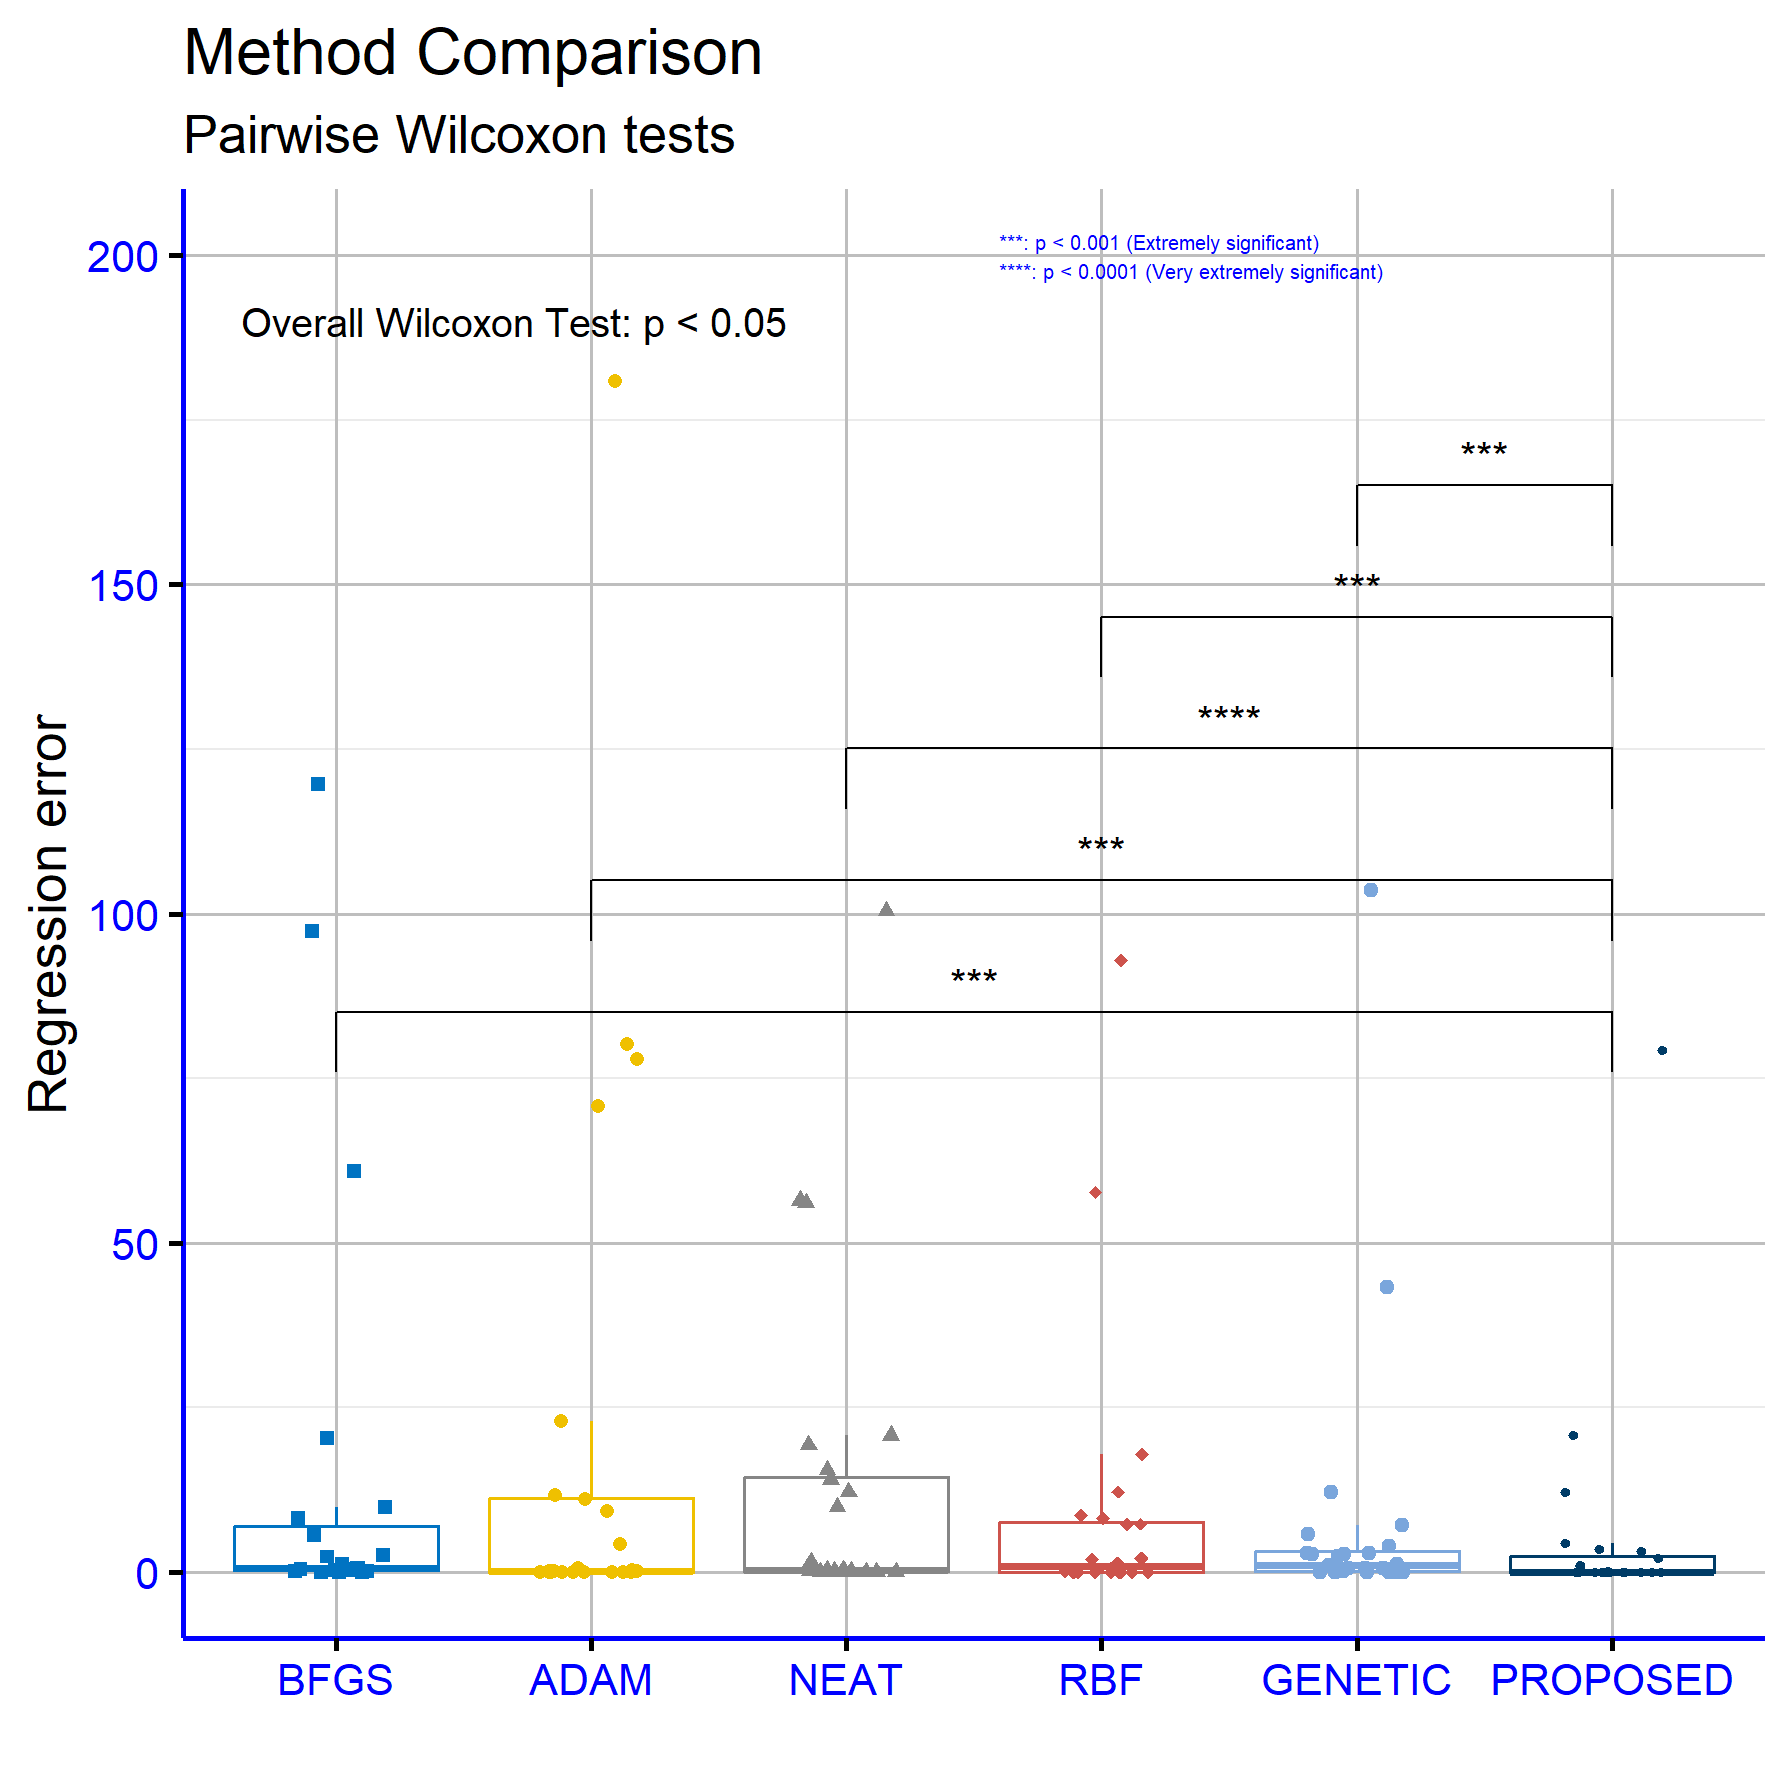
\includegraphics[scale=0.5]{stat2}

\caption{Statistical comparison for the experimental results obtained by the
application of the mentioned machine learning methods on the regression
datasets.\protect\label{fig:stat2}}

\end{figure}

An addition experiment was performed using a variety of values for
the initialization factor $I_{0}$ and the regression datasets. The
average regression error from this experiment and for each value of
$I_{0}$ is depicted graphically in Figure \ref{fig:experI0}.

\begin{figure}[H]
\begin{centering}
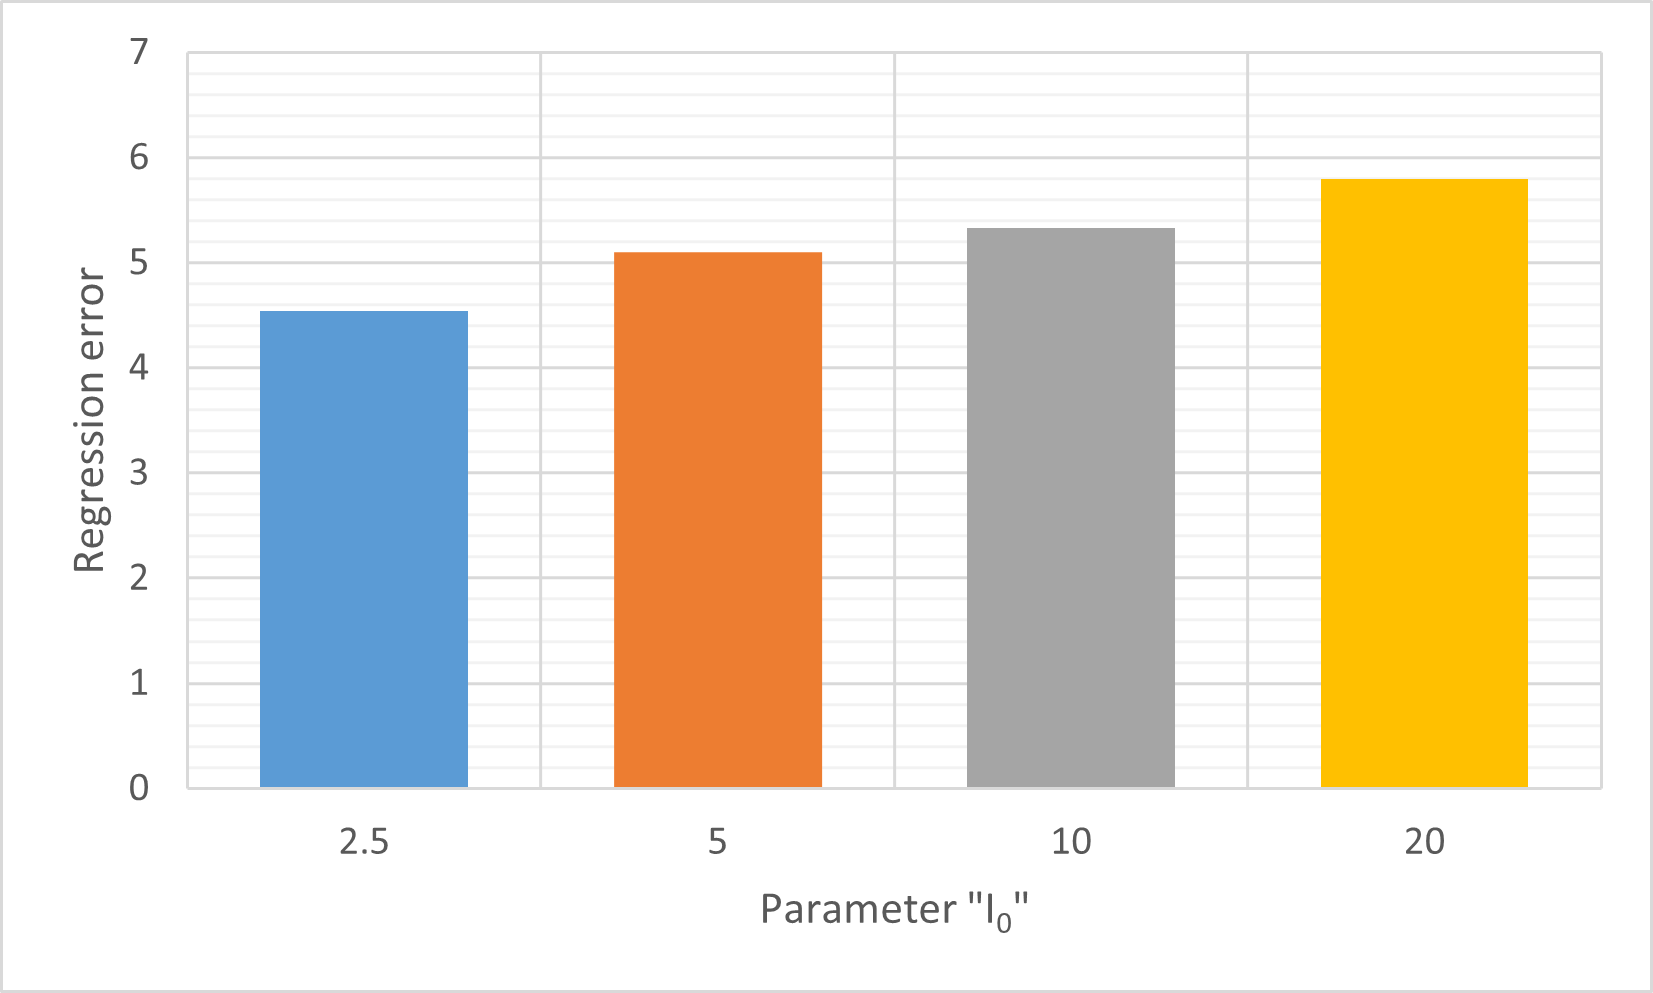
\includegraphics[scale=0.5]{plot_i0}
\par\end{centering}
\caption{Experiments using different values of the initialization factor $I_{0}$
and the used regression datasets.\protect\label{fig:experI0}}

\end{figure}
The obtained regression error remains low for lower value of the initialization
factor and increases as this factor gets higher values. This means
that initializing the parameters of the neural network in a value
interval with smaller extreme values \LyXZeroWidthSpace and a smaller
range gives the artificial neural network better generalization capabilities.

Also, a similar experiment was conducted using different values of
the scale factor $f$ and the utilized regression datasets. The average
regression error for this experiment is outlined graphically in Figure
\ref{fig:experF}.

\begin{figure}[H]
\begin{centering}
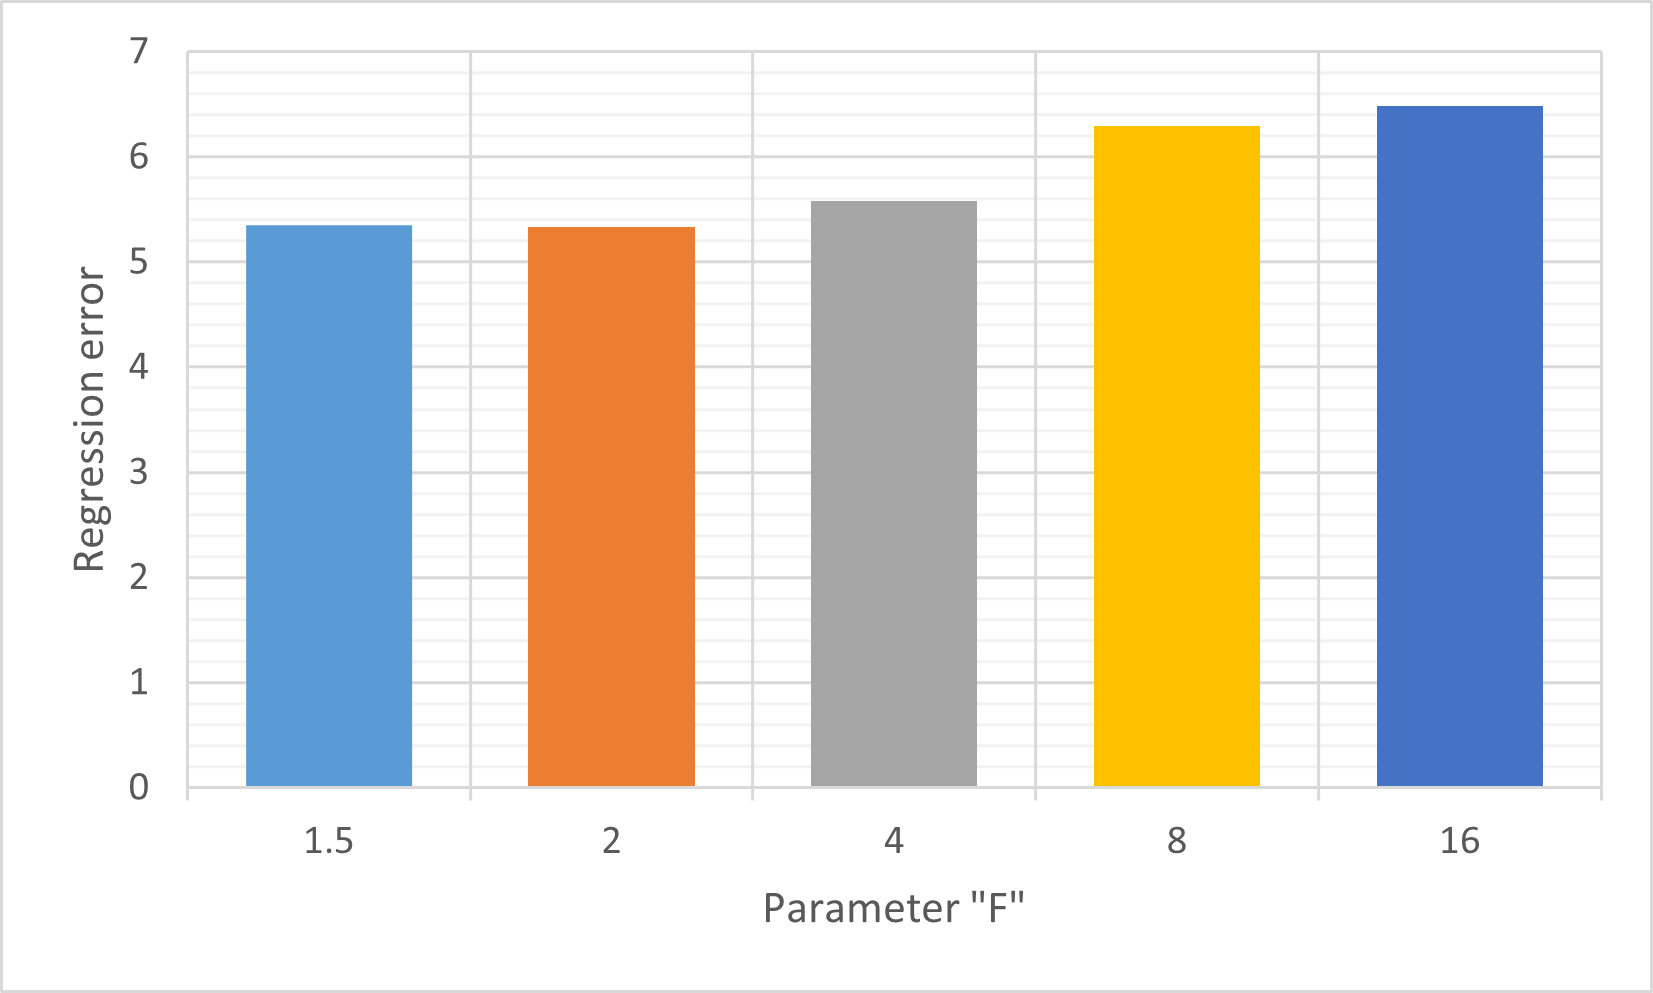
\includegraphics[scale=0.5]{plot_f}
\par\end{centering}
\caption{The average regression error obtained by the usage of the proposed
method on the regression datasets for a variety of values of the scale
factor $f$.\protect\label{fig:experF}}

\end{figure}
As it can observed, as the scale factor increases the average regression
error increases also. The conclusion from this experiment is that
the artificial neural network is able to generalize more efficiently
when its parameter values \LyXZeroWidthSpace are limited to a smaller
range of values \LyXZeroWidthSpace than those identified in the first
phase.

\section{Conclusions\protect\label{sec:Conclusions}}

The proposed method for training artificial neural networks is based
on the application of genetic algorithms in three distinct phases,with
the primary objective of efficient training and minimizing overfitting,
a common challenge in modern optimization techniques. The first phase
focuses on identifying an initial interval for the values of the network.
This phase is crucial as it sets the initial positioning of the parameters
within a range that avoids excessively large values, which could limit
the model’s generalization capability. The proposed value range is
determined using a genetic algorithm that incorporates a modified
error calculation, penalizing large parameter values. This step reduces
the risk of overfitting to the training data, enhancing the model's
capacity to respond effectively to unseen data. In the second phase,
the method employs an optimized genetic algorithm to identify the
ideal parameter value bounds within the initially defined range. This
process makes the method particularly effective as it focuses on intervals
already evaluated as suitable while incorporating representative samples
from the initial value range to assess accuracy. The use of genetic
algorithms allows for gradual and adaptive improvement, eliminating
local minima a frequent issue in traditional optimization methods.
The third phase focuses on training the neural network within the
optimized parameter bounds. In this phase, a genetic algorithm used
to minimize the training error, followed by a local optimization step
using the BFGS method. This local optimization ensures further accuracy
improvement, fully utilizing the model's potential. The experiments
conducted demonstrate the clear superiority of the proposed method
compared to other established techniques. For classification datasets,
the method achieved significantly lower error rates compared to techniques
like ADAM, BFGS, and NEAT. For example, in datasets such as Dermatology
and HouseVotes, the error rate was nearly halved compared to alternative
methods. Similar results were observed for regression datasets, where
the method achieved the highest accuracy across nearly all datasets.
The lowest average error achieved highlights its consistent and versatile
performance. A notable innovation of the method is its approach to
tackling overfitting. The genetic algorithms enable exploration across
a wide range of values without being constrained to local minima.
Simultaneously, the incorporation of penalties for large parameter
values prevents excessive adaptation to the training data. This is
particularly important as overfitting often limits the performance
of artificial neural networks when applied to unseen data. Experiments
with varying initial parameters, such as the initialization factor
and the scale factor, provide valuable insights into model configuration.
For instance, smaller initial value ranges contributed to better generalization,
while larger scale factor values led to higher error, emphasizing
the importance of tighter parameter bounds. This indicates that careful
parameter selection is critical for overall performance. 

The proposed method paves new paths for the application of genetic
algorithms in training process of neural networks. Its adaptive nature
makes it suitable for a wide range of applications, from medical diagnosis
and forecasting of physical phenomena to the optimization of industrial
processes. Future steps could include its application in deep learning
networks, the integration of hybrid methods combining genetic algorithms
with other optimization techniques, and the use of distributed computing
environments to accelerate training. This approach has the potential
to become a benchmark for effective and reliable training of artificial
neural networks.

\vspace{6pt}


\authorcontributions{V.C. and I.G.T. conducted the experiments, employing several datasets
and provided the comparative experiments. V.C. performed the statistical
analysis and prepared the manuscript. All authors have read and agreed
to the published version of the manuscript.}

\funding{This research received no external funding.}

\institutionalreview{Not applicable.}

\informedconsent{Not applicable.}

\acknowledgments{This research has been financed by the European Union : Next Generation
EU through the Program Greece 2.0 National Recovery and Resilience
Plan , under the call RESEARCH -- CREATE -- INNOVATE, project name
“iCREW: Intelligent small craft simulator for advanced crew training
using Virtual Reality techniques\textquotedbl{} (project code:TAEDK-06195).}

\conflictsofinterest{The authors declare no conflicts of interest.}

\begin{adjustwidth}{-\extralength}{0cm}{}

\reftitle{References}
\begin{thebibliography}{99}
\bibitem[(2018)]{nn1}Abiodun, O. I., Jantan, A., Omolara, A. E.,
Dada, K. V., Mohamed, N. A., \& Arshad, H. (2018). State-of-the-art
in artificial neural network applications: A survey. Heliyon, 4(11).

\bibitem{nn2}Suryadevara, S., \& Yanamala, A. K. Y. (2021). A Comprehensive
Overview of Artificial Neural Networks: Evolution, Architectures,
and Applications. Revista de Inteligencia Artificial en Medicina,
12(1), 51-76.

\bibitem{nnc}I.G. Tsoulos, D. Gavrilis, E. Glavas, Neural network
construction and training using grammatical evolution, Neurocomputing
\textbf{72}, pp. 269-277, 2008.

\bibitem{activation_spline}S. Guarnieri, F. Piazza, A. Uncini, Multilayer
feedforward networks with adaptive spline activation function, IEEE
Transactions on Neural Networks \textbf{10}, pp. 672-683, 1999. 

\bibitem{activation_trained}Ö.F. Ertuğrul, A novel type of activation
function in artificial neural networks: Trained activation function,
Neural Networks \textbf{99}, pp. 148-157, 2018.

\bibitem{activation_review}A. D. Rasamoelina, F. Adjailia, P. Sinčák,
A Review of Activation Function for Artificial Neural Network, In:
2020 IEEE 18th World Symposium on Applied Machine Intelligence and
Informatics (SAMI), Herlany, Slovakia, pp. 281-286, 2020.

\bibitem{nn_image}M. Egmont-Petersen, D. de Ridder, H. Handels, Image
processing with neural networks---a review, Pattern Recognition \textbf{35},
pp. 2279-2301, 2002.

\bibitem{nn_timeseries}G.Peter Zhang, Time series forecasting using
a hybrid ARIMA and neural network model, Neurocomputing \textbf{50},
pp. 159-175, 2003.

\bibitem{nn_credit}Z. Huang, H. Chen, C.-Jung Hsu, W.-Hwa Chen, S.
Wu, Credit rating analysis with support vector machines and neural
networks: a market comparative study, Decision Support Systems \textbf{37},
pp. 543-558, 2004.

\bibitem{nnphysics1}P. Baldi, K. Cranmer, T. Faucett et al, Parameterized
neural networks for high-energy physics, Eur. Phys. J. C \textbf{76},
2016.

\bibitem{nnphysics2}Baldi, P., Cranmer, K., Faucett, T., Sadowski,
P., \& Whiteson, D. (2016). Parameterized neural networks for high-energy
physics. The European Physical Journal C, 76(5), 1-7.

\bibitem{nnmed1}Igor I. Baskin, David Winkler and Igor V. Tetko,
A renaissance of neural networks in drug discovery, Expert Opinion
on Drug Discovery \textbf{11}, pp. 785-795, 2016.

\bibitem{nnmed2}Ronadl Bartzatt, Prediction of Novel Anti-Ebola Virus
Compounds Utilizing Artificial Neural Network (ANN), Chemistry Faculty
Publications \textbf{49}, pp. 16-34, 2018.

\bibitem{nn_mech1}K. Peta, J. Żurek, Prediction of air leakage in
heat exchangers for automotive applications using artificial neural
networks, In: 2018 9th IEEE Annual Ubiquitous Computing, Electronics
\& Mobile Communication Conference (UEMCON), New York, NY, USA, pp.
721-725, 2018.

\bibitem{bpnn1}Vora, K., \& Yagnik, S. (2014). A survey on backpropagation
algorithms for feedforward neural networks. International Journal
of Engineering Development and Research, 1(3), 193-197.

\bibitem{bpnn2}K. Vora, S. Yagnik, A survey on backpropagation algorithms
for feedforward neural networks, International Journal of Engineering
Development and Research \textbf{1}, pp. 193-197, 2014.

\bibitem{rpropnn-1}Pajchrowski, T., Zawirski, K., \& Nowopolski,
K. (2014). Neural speed controller trained online by means of modified
RPROP algorithm. IEEE transactions on industrial informatics, 11(2),
560-568.

\bibitem{rpropnn-2}Hermanto, R. P. S., \& Nugroho, A. (2018). Waiting-time
estimation in bank customer queues using RPROP neural networks. Procedia
Computer Science, 135, 35-42.

\bibitem{nn_adam}D. P. Kingma, J. L. Ba, ADAM: a method for stochastic
optimization, in: Proceedings of the 3rd International Conference
on Learning Representations (ICLR 2015), pp. 1--15, 2015.

\bibitem{geneticnn1}Reynolds, J., Rezgui, Y., Kwan, A., \& Piriou,
S. (2018). A zone-level, building energy optimisation combining an
artificial neural network, a genetic algorithm, and model predictive
control. Energy, 151, 729-739.

\bibitem{psonn}Das, G., Pattnaik, P. K., \& Padhy, S. K. (2014).
Artificial neural network trained by particle swarm optimization for
non-linear channel equalization. Expert Systems with Applications,
41(7), 3491-3496.

\bibitem{nn_siman}Sexton, R. S., Dorsey, R. E., \& Johnson, J. D.
(1999). Beyond backpropagation: using simulated annealing for training
neural networks. Journal of Organizational and End User Computing
(JOEUC), 11(3), 3-10.

\bibitem{weight_de1}Wang, L., Zeng, Y., \& Chen, T. (2015). Back
propagation neural network with adaptive differential evolution algorithm
for time series forecasting. Expert Systems with Applications, 42(2),
855-863.

\bibitem{nn_abc}Karaboga, D., \& Akay, B. (2007, June). Artificial
bee colony (ABC) algorithm on training artificial neural networks.
In 2007 IEEE 15th Signal Processing and Communications Applications
(pp. 1-4). IEEE.

\bibitem{tabunn}R.S. Sexton, B. Alidaee, R.E. Dorsey, J.D. Johnson,
Global optimization for artificial neural networks: A tabu search
application. European Journal of Operational Research \textbf{106},
pp. 570-584, 1998.

\bibitem{nn_hybrid}J.-R. Zhang, J. Zhang, T.-M. Lok, M.R. Lyu, A
hybrid particle swarm optimization--back-propagation algorithm for
feedforward neural network training, Applied Mathematics and Computation
\textbf{185}, pp. 1026-1037, 2007.

\bibitem{nn_cascade}G. Zhao, T. Wang, Y. Jin, C. Lang, Y. Li, H.
Ling, The Cascaded Forward algorithm for neural network training,
Pattern Recognition \textbf{161}, 111292, 2025.

\bibitem{nn_gpu1}K-Su Oh, K. Jung, GPU implementation of neural networks,
Pattern Recognition \textbf{37}, pp. 1311-1314, 2004.

\bibitem{nn_gpu2}M. Zhang, K. Hibi, J. Inoue, GPU-accelerated artificial
neural network potential for molecular dynamics simulation, Computer
Physics Communications \textbf{285}, 108655, 2023. 

\bibitem{nnsharing1}S.J. Nowlan and G.E. Hinton, Simplifying neural
networks by soft weight sharing, Neural Computation 4, pp. 473-493,
1992.

\bibitem{nnsharing2}Nowlan, S. J., \& Hinton, G. E. (2018). Simplifying
neural networks by soft weight sharing. In The mathematics of generalization
(pp. 373-394). CRC Press.

\bibitem{nnprunning1}S.J. Hanson and L.Y. Pratt, Comparing biases
for minimal network construction with back propagation, In D.S. Touretzky
(Ed.), Advances in Neural Information Processing Systems, Volume 1,
pp. 177-185, San Mateo, CA: Morgan Kaufmann, 1989.

\bibitem{nnprunning2}M. Augasta and T. Kathirvalavakumar, Pruning
algorithms of neural networks --- a comparative study, Central European
Journal of Computer Science, 2003.

\bibitem{nnearly1}Lutz Prechelt, Automatic early stopping using cross
validation: quantifying the criteria, Neural Networks \textbf{11},
pp. 761-767, 1998.

\bibitem{nnearly2}X. Wu and J. Liu, A New Early Stopping Algorithm
for Improving Neural Network Generalization, 2009 Second International
Conference on Intelligent Computation Technology and Automation, Changsha,
Hunan, 2009, pp. 15-18.

\bibitem{nndecay1}N. K. Treadgold and T. D. Gedeon, Simulated annealing
and weight decay in adaptive learning: the SARPROP algorithm,IEEE
Transactions on Neural Networks \textbf{9}, pp. 662-668, 1998.

\bibitem{nndecay2}M. Carvalho and T. B. Ludermir, Particle Swarm
Optimization of Feed-Forward Neural Networks with Weight Decay, 2006
Sixth International Conference on Hybrid Intelligent Systems (HIS'06),
Rio de Janeiro, Brazil, 2006, pp. 5-5.

\bibitem{nn_arch1}J. Arifovic, R. Gençay, Using genetic algorithms
to select architecture of a feedforward artificial neural network,
Physica A: Statistical Mechanics and its Applications \textbf{289},
pp. 574-594, 2001.

\bibitem{nn_arch2}P.G. Benardos, G.C. Vosniakos, Optimizing feedforward
artificial neural network architecture, Engineering Applications of
Artificial Intelligence \textbf{20}, pp. 365-382, 2007.

\bibitem{nn_arch3}B.A. Garro, R.A. Vázquez, Designing Artificial
Neural Networks Using Particle Swarm Optimization Algorithms, Computational
Intelligence and Neuroscience, 369298, 2015. 

\bibitem[(2001)]{nn_ereinf}Siebel, N. T., \& Sommer, G. (2007). Evolutionary
reinforcement learning of artificial neural networks. International
Journal of Hybrid Intelligent Systems, 4(3), 171-183.

\bibitem[(2001)]{nn_reinf}Jaafra, Y., Laurent, J. L., Deruyver, A.,
\& Naceur, M. S. (2019). Reinforcement learning for neural architecture
search: A review. Image and Vision Computing, 89, 57-66.

\bibitem[(2001)]{nn_param_sharing}Pham, H., Guan, M., Zoph, B., Le,
Q., \& Dean, J. (2018, July). Efficient neural architecture search
via parameters sharing. In International conference on machine learning
(pp. 4095-4104). PMLR.

\bibitem[(2001)]{nn_snas}Xie, S., Zheng, H., Liu, C., \& Lin, L.
(2018). SNAS: stochastic neural architecture search. arXiv preprint
arXiv:1812.09926.

\bibitem[(2001)]{nn_bayes}Zhou, H., Yang, M., Wang, J., \& Pan, W.
(2019, May). Bayesnas: A bayesian approach for neural architecture
search. In International conference on machine learning (pp. 7603-7613).
PMLR.

\bibitem[(2013)]{weight_gpu2}A.A. Huqqani, E. Schikuta, S. Ye Peng
Chen, Multicore and GPU Parallelization of Neural Networks for Face
Recognition, Procedia Computer Science \textbf{18}, pp. 349-358, 2013.

\bibitem{kaelo}P. Kaelo, M.M. Ali, Integrated crossover rules in
real coded genetic algorithms, European Journal of Operational Research
\textbf{176}, pp. 60-76, 2007.

\bibitem{powell}M.J.D Powell, A Tolerant Algorithm for Linearly Constrained
Optimization Calculations, Mathematical Programming \textbf{45}, pp.
547-566, 1989. 

\bibitem[(1989)]{uci} M. Kelly, R. Longjohn, K. Nottingham, The UCI
Machine Learning Repository, https://archive.ics.uci.edu.

\bibitem{Keel}J. Alcalá-Fdez, A. Fernandez, J. Luengo, J. Derrac,
S. García, L. Sánchez, F. Herrera. KEEL Data-Mining Software Tool:
Data Set Repository, Integration of Algorithms and Experimental Analysis
Framework. Journal of Multiple-Valued Logic and Soft Computing 17,
pp. 255-287, 2011.

\bibitem{appendicitis}Weiss, Sholom M. and Kulikowski, Casimir A.,
Computer Systems That Learn: Classification and Prediction Methods
from Statistics, Neural Nets, Machine Learning, and Expert Systems,
Morgan Kaufmann Publishers Inc, 1991.

\bibitem[Tzimourta(2018)]{alcohol}Tzimourta, K.D.; Tsoulos, I.; Bilero,
I.T.; Tzallas, A.T.; Tsipouras, M.G.; Giannakeas, N. Direct Assessment
of Alcohol Consumption in Mental State Using Brain Computer Interfaces
and Grammatical Evolution. Inventions 2018, 3, 51.

\bibitem[Quinlan(2018)]{australian}J.R. Quinlan, Simplifying Decision
Trees. International Journal of Man-Machine Studies \textbf{27}, pp.
221-234, 1987. 

\bibitem{balance}T. Shultz, D. Mareschal, W. Schmidt, Modeling Cognitive
Development on Balance Scale Phenomena, Machine Learning \textbf{16},
pp. 59-88, 1994.

\bibitem[(2004)]{cleveland1}Z.H. Zhou,Y. Jiang, NeC4.5: neural ensemble
based C4.5,\textquotedbl{} in IEEE Transactions on Knowledge and Data
Engineering \textbf{16}, pp. 770-773, 2004.

\bibitem{cleveland2}R. Setiono , W.K. Leow, FERNN: An Algorithm for
Fast Extraction of Rules from Neural Networks, Applied Intelligence
\textbf{12}, pp. 15-25, 2000.

\bibitem[(1998)]{dermatology}G. Demiroz, H.A. Govenir, N. Ilter,
Learning Differential Diagnosis of Eryhemato-Squamous Diseases using
Voting Feature Intervals, Artificial Intelligence in Medicine. \textbf{13},
pp. 147--165, 1998.

\bibitem[(1977)]{hayes-roth}B. Hayes-Roth, B., F. Hayes-Roth. Concept
learning and the recognition and classification of exemplars. Journal
of Verbal Learning and Verbal Behavior \textbf{16}, pp. 321-338, 1977.

\bibitem[(1997)]{heart}I. Kononenko, E. Šimec, M. Robnik-Šikonja,
Overcoming the Myopia of Inductive Learning Algorithms with RELIEFF,
Applied Intelligence \textbf{7}, pp. 39--55, 1997

\bibitem[(2002)]{housevotes}R.M. French, N. Chater, Using noise to
compute error surfaces in connectionist networks: a novel means of
reducing catastrophic forgetting, Neural Comput. \textbf{14}, pp.
1755-1769, 2002.

\bibitem[(2004)]{ion1}J.G. Dy , C.E. Brodley, Feature Selection for
Unsupervised Learning, The Journal of Machine Learning Research \textbf{5},
pp 845--889, 2004.

\bibitem{ion2}S. J. Perantonis, V. Virvilis, Input Feature Extraction
for Multilayered Perceptrons Using Supervised Principal Component
Analysis, Neural Processing Letters \textbf{10}, pp 243--252, 1999.

\bibitem[(2002)]{liver} J. Garcke, M. Griebel, Classification with
sparse grids using simplicial basis functions, Intell. Data Anal.
\textbf{6}, pp. 483-502, 2002.

\bibitem{liver1}J. Mcdermott, R.S. Forsyth, Diagnosing a disorder
in a classification benchmark, Pattern Recognition Letters \textbf{73},
pp. 41-43, 2016.

\bibitem[(2002)]{lymography}G. Cestnik, I. Konenenko, I. Bratko,
Assistant-86: A Knowledge-Elicitation Tool for Sophisticated Users.
In: Bratko, I. and Lavrac, N., Eds., Progress in Machine Learning,
Sigma Press, Wilmslow, pp. 31-45, 1987. 

\bibitem[(2007)]{mammographic}M. Elter, R. Schulz-Wendtland, T. Wittenberg,
The prediction of breast cancer biopsy outcomes using two CAD approaches
that both emphasize an intelligible decision process, Med Phys. \textbf{34},
pp. 4164-72, 2007.

\bibitem[(2007)]{parkinsons1}M.A. Little, P.E. McSharry, S.J Roberts
et al, Exploiting Nonlinear Recurrence and Fractal Scaling Properties
for Voice Disorder Detection. BioMed Eng OnLine \textbf{6}, 23, 2007.

\bibitem{parkinsons2}M.A. Little, P.E. McSharry, E.J. Hunter, J.
Spielman, L.O. Ramig, Suitability of dysphonia measurements for telemonitoring
of Parkinson's disease. IEEE Trans Biomed Eng. \textbf{56}, pp. 1015-1022,
2009.

\bibitem[(2007)]{pima}J.W. Smith, J.E. Everhart, W.C. Dickson, W.C.
Knowler, R.S. Johannes, Using the ADAP learning algorithm to forecast
the onset of diabetes mellitus, In: Proceedings of the Symposium on
Computer Applications and Medical Care IEEE Computer Society Press,
pp.261-265, 1988.

\bibitem[(2007)]{popfailures}D.D. Lucas, R. Klein, J. Tannahill,
D. Ivanova, S. Brandon, D. Domyancic, Y. Zhang, Failure analysis of
parameter-induced simulation crashes in climate models, Geoscientific
Model Development \textbf{6}, pp. 1157-1171, 2013.

\bibitem[(2007)]{regions2}N. Giannakeas, M.G. Tsipouras, A.T. Tzallas,
K. Kyriakidi, Z.E. Tsianou, P. Manousou, A. Hall, E.C. Karvounis,
V. Tsianos, E. Tsianos, A clustering based method for collagen proportional
area extraction in liver biopsy images (2015) Proceedings of the Annual
International Conference of the IEEE Engineering in Medicine and Biology
Society, EMBS, 2015-November, art. no. 7319047, pp. 3097-3100. 

\bibitem[(2007)]{saheart}T. Hastie, R. Tibshirani, Non-parametric
logistic and proportional odds regression, JRSS-C (Applied Statistics)
\textbf{36}, pp. 260--276, 1987.

\bibitem{segment}M. Dash, H. Liu, P. Scheuermann, K. L. Tan, Fast
hierarchical clustering and its validation, Data \& Knowledge Engineering
\textbf{44}, pp 109--138, 2003.

\bibitem[(1988)]{sonar}Gorman, R.P.; Sejnowski, T.J. Analysis of
Hidden Units in a Layered Network Trained to Classify Sonar Targets.
Neural Netw. 1988, 1, 75--89.

\bibitem[(2007)]{student}P. Cortez, A. M. Gonçalves Silva, Using
data mining to predict secondary school student performance, In Proceedings
of 5th FUture BUsiness TEChnology Conference (FUBUTEC 2008) (pp. 5--12).
EUROSIS-ETI, 2008.

\bibitem[(2007)]{transfusion}I-Cheng Yeh, King-Jang Yang, Tao-Ming
Ting, Knowledge discovery on RFM model using Bernoulli sequence, Expert
Systems with Applications \textbf{36}, pp. 5866-5871, 2009.

\bibitem[(2007)]{wdbc1}Jeyasingh, S., \& Veluchamy, M. (2017). Modified
bat algorithm for feature selection with the Wisconsin diagnosis breast
cancer (WDBC) dataset. Asian Pacific journal of cancer prevention:
APJCP, 18(5), 1257.

\bibitem[(2007)]{wdbc2}Alshayeji, M. H., Ellethy, H., \& Gupta, R.
(2022). Computer-aided detection of breast cancer on the Wisconsin
dataset: An artificial neural networks approach. Biomedical signal
processing and control, 71, 103141.

\bibitem[(2007)]{wine1}M. Raymer, T.E. Doom, L.A. Kuhn, W.F. Punch,
Knowledge discovery in medical and biological datasets using a hybrid
Bayes classifier/evolutionary algorithm. IEEE transactions on systems,
man, and cybernetics. Part B, Cybernetics : a publication of the IEEE
Systems, Man, and Cybernetics Society, \textbf{33} , pp. 802-813,
2003.

\bibitem{wine2}P. Zhong, M. Fukushima, Regularized nonsmooth Newton
method for multi-class support vector machines, Optimization Methods
and Software \textbf{22}, pp. 225-236, 2007.

\bibitem[(2007)]{eeg1}R. G. Andrzejak, K. Lehnertz, F.Mormann, C.
Rieke, P. David, and C. E. Elger, “Indications of nonlinear deterministic
and finite-dimensional structures in time series of brain electrical
activity: dependence on recording region and brain state,” Physical
Review E, vol. 64, no. 6, Article ID 061907, 8 pages, 2001. 

\bibitem{eeg2}A. T. Tzallas, M. G. Tsipouras, and D. I. Fotiadis,
“Automatic Seizure Detection Based on Time-Frequency Analysis and
Artificial Neural Networks,” Computational Intelligence and Neuroscience,
vol. 2007, Article ID 80510, 13 pages, 2007. doi:10.1155/2007/80510

\bibitem[(2007)]{zoo}M. Koivisto, K. Sood, Exact Bayesian Structure
Discovery in Bayesian Networks, The Journal of Machine Learning Research\textbf{
5}, pp. 549--573, 2004.

\bibitem[(2007)]{abalone}Nash, W.J.; Sellers, T.L.; Talbot, S.R.;
Cawthor, A.J.; Ford, W.B. The Population Biology of Abalone (\_Haliotis\_
species) in Tasmania. I. Blacklip Abalone (\_H. rubra\_) from the
North Coast and Islands of Bass Strait, Sea Fisheries Division; Technical
Report No. 48; Department of Primary Industry and Fisheries, Tasmania:
Hobart, Australia, 1994; ISSN 1034-3288

\bibitem[(2007)]{airfoil}Brooks, T.F.; Pope, D.S.; Marcolini, A.M.
Airfoil Self-Noise and Prediction. Technical Report, NASA RP-1218.
July 1989. Available online: https://ntrs.nasa.gov/citations/19890016302
(accessed on 14 November 2024).

\bibitem[(2007)]{concrete}I.Cheng Yeh, Modeling of strength of high
performance concrete using artificial neural networks, Cement and
Concrete Research. \textbf{28}, pp. 1797-1808, 1998. 

\bibitem{friedman}Friedman, J. (1991): Multivariate Adaptative Regression
Splines. Annals of Statistics, 19:1, 1-{}-141. 

\bibitem[(2007)]{housing}D. Harrison and D.L. Rubinfeld, Hedonic
prices and the demand for clean ai, J. Environ. Economics \& Management
\textbf{5}, pp. 81-102, 1978.

\bibitem[(1988)]{ntdataset}Mackowiak, P.A., Wasserman, S.S., Levine,
M.M., 1992. A critical appraisal of 98.6 degrees f, the upper limit
of the normal body temperature, and other legacies of Carl Reinhold
August Wunderlich. J. Amer. Med. Assoc. 268, 1578--1580

\bibitem[(1988)]{pydataset}R.D. King, S. Muggleton, R. Lewis, M.J.E.
Sternberg, Proc. Nat. Acad. Sci. USA \textbf{89}, pp. 11322--11326,
1992. 

\bibitem[(2025)]{optimus}I.G. Tsoulos, V. Charilogis, G. Kyrou, V.N.
Stavrou, A. Tzallas, Journal of Open Source Software \textbf{10},
7584, 2025.

\bibitem[(2025)]{neat}K. O. Stanley, R. Miikkulainen, Evolving Neural
Networks through Augmenting Topologies, Evolutionary Computation \textbf{10},
pp. 99-127, 2002.

\bibitem[(1991)]{rbf1}J. Park and I. W. Sandberg, Universal Approximation
Using Radial-Basis-Function Networks, Neural Computation \textbf{3},
pp. 246-257, 1991.

\bibitem{rbf2}G.A. Montazer, D. Giveki, M. Karami, H. Rastegar, Radial
basis function neural networks: A review. Comput. Rev. J \textbf{1},
pp. 52-74, 2018.

\end{thebibliography}
%%%%%%%%%%%%%%%%%%%%%%%%%%%%%%%%%%%%%%%%%%
%% for journal Sci
%\reviewreports{\\
%Reviewer 1 comments and authors' response\\
%Reviewer 2 comments and authors' response\\
%Reviewer 3 comments and authors' response
%}
%%%%%%%%%%%%%%%%%%%%%%%%%%%%%%%%%%%%%%%%%%

\PublishersNote{}

\end{adjustwidth}{}
\end{document}
